\graphicspath{{img/thermalisation/}}

\chapter{Dark Matter Induced Heating of Neutron Stars}
\label{chapter:heating}

\begin{synopsis}
This chapter is based on the results of Ref.~\cite{Bell:2023ysh_dec_ThermalizationAnnihilationDark}, which discusses the thermalisation and annihilation of dark matter in neutron stars. We consider the extent to which dark matter can heat up a neutron star through the scatterings and annihilations that occur after its capture.  We apply the formalism presented in the previous chapters for dark matter scattering in a degenerate media to determine the timescales required to kinetically heat the star by depositing 99\% of its initial energy and, in addition, the time required for it to thermalise. Furthermore, we compute the capture-annihilation equilibrium timescale, and hence determine the maximal heating that can be achieved within the lifetime of the star. In these calculations, we account for the population of the dark matter that has yet to fully thermalise. 
\end{synopsis}




%%%%%%%%%%%%%%%%%%%%%%%%%%%%%%%%%%%%%%%%%%%%%%%%%%%%%%%%%%%%%%%%%%%%%%%%%%%%%%%%%%%%
%%%%%%%%%%%%%%%%%%%%%%%%%%%%%%%%%%%%%%%%%%%%%%%%%%%%%%%%%%%%%%%%%%%%%%%%%%%%%%%%%%%%
\section{Introduction}
\label{ch6:sec:introduction}
%%%%%%%%%%%%%%%%%%%%%%%%%%%%%%%%%%%%%%%%%%%%%%%%%%%%%%%%%%%%%%%%%%%%%%%%%%%%%%%%%%%%
%%%%%%%%%%%%%%%%%%%%%%%%%%%%%%%%%%%%%%%%%%%%%%%%%%%%%%%%%%%%%%%%%%%%%%%%%%%%%%%%%%%%

It was recently pointed out that old, isolated NSs in the Solar neighbourhood could be heated by DM capture~\cite{Baryakhtar:2017dbj_sep_DarkKineticHeating}, leading to a temperature increase of $\sim 2000\K$. 
At ages greater than $\sim 10\Myr$, isolated NSs are expected to cool to temperatures below this, provided they are not reheated by accretion of standard matter or by internal heating mechanisms~\cite{Gonzalez:2010ta_Internalheatingold}.
As a result, the observation of a local NS with a temperature $\mathcal{O}(1000\K)$ could provide stringent constraints on DM interactions. Importantly,
NS temperatures in this range would result in near-infrared emission, potentially detectable by future telescopes.


There are two distinct contributions to this heating: 
\begin{enumerate}
    \item Kinetic heating, where the DM kinetic energy is deposited in the NS medium. 
    \item Annihilation heating, where the DM rest mass energy is deposited through the annihilation of DM to particles that are trapped in the star.
\end{enumerate}


The kinetic heating occurs as follows: The initial scattering interaction, which leads to gravitational capture of the DM particle, transfers only a small portion of the DM kinetic energy to the star.  The rest of the kinetic energy is transferred through subsequent scattering interactions of the gravitationally bound DM until, eventually, the DM thermalizes with constituents in the centre of the star.  In general, a large number of collisions are typically required for full thermalization.  Moreover, if the scattering cross-section is momentum suppressed in the non-relativistic limit, the time between collisions, and hence the time required to achieve full thermalization, can become very large, larger than the age of the Universe.  Importantly, we shall see that even in cases where the full thermalization process is slow, {\it the majority of the kinetic energy is deposited very quickly.} 


DM annihilation occurs in a region very close to the centre of the star, where the thermalized DM accumulates.  The annihilation rate will increase as the DM abundance in the star grows until, eventually, a state of equilibrium between capture and annihilation is reached.  When this occurs, the annihilation heating is maximized.  The complete thermalization of the DM will result in a smaller, denser sphere of thermalized DM in the centre of the star, assisting in annihilation.  However, we shall find that {\it capture-annihilation equilibrium, and hence maximal annihilation heating, can be achieved \it without full thermalization}.


The thermalization process was previously examined in refs.~\cite{Bertoni:2013bsa_dec_DarkMatterThermalization,Garani:2020wge_Observingthermalizationdark} for a subset of interaction types. These previous studies did not consider the importance of annihilation heating from partially thermalized DM. In this chapter, we present a detailed calculation of the timescales required for thermalization and capture-annihilation equilibrium, utilising the improved treatment of DM capture in NSs presented in the previous chapters. We perform these calculations for a full set of DM-nucleon interaction types, parameterized by a set of Effective Field Theory (EFT) operators for fermionic DM.  This includes operators for which either the scattering cross-section or the annihilation cross-section is suppressed in the non-relativistic limit.  By properly accounting for the annihilation of partially thermalized DM, we show that full kinetic plus annihilation heating can be achieved for most of the interesting parameter space on a short timescale.

%%%%%%%%%%%%%%%%%%%%%%%%%%%%%%%%%%%%%%%%%%%%%%%%%%%%%%%%%%%%%%%%%%%%%%%%%%%%%%%%%%%%
%%%%%%%%%%%%%%%%%%%%%%%%%%%%%%%%%%%%%%%%%%%%%%%%%%%%%%%%%%%%%%%%%%%%%%%%%%%%%%%%%%%%
\section{Neutron Star Temperature from Dark Matter  Heating}
\label{ch6:sec:temperature}
%%%%%%%%%%%%%%%%%%%%%%%%%%%%%%%%%%%%%%%%%%%%%%%%%%%%%%%%%%%%%%%%%%%%%%%%%%%%%%%%%%%%
%%%%%%%%%%%%%%%%%%%%%%%%%%%%%%%%%%%%%%%%%%%%%%%%%%%%%%%%%%%%%%%%%%%%%%%%%%%%%%%%%%%%



% In the absence of any source of heat, neutron stars will spend their lifetimes cooling through the emission of neutrinos from the within the core, as well as photons from the crust~\cite{Yakovlev:1999sk_Coolingneutronstars,Yakovlev:2000jp_Neutrinoemissionneutron,Yakovlev:2004iq_Neutronstarcooling}, with the neutrino emission dominating the cooling at early times, $\tstar \lesssim 10^5\yrs$. We denote the individual contributions to the total luminosity of the star as $L_\nu$ and $L_\gamma$ for neutrino and photon emission respectively. 
% % The luminosity of the star as seen by a distant observer will be redshifted by the NS gravitational potential, such that $L_i^\infty = \sqrt{B(\Rstar)} L_i$. The observed temperature will be similarly redshifted, $\Tstar^\inf = \sqrt{B(\Rstar)} \Tstar$. Assuming no additional heating sources, $\Tstar^\infty$ will evolve according to
%  \begin{equation}
%     C_V\frac{d T^\infty_\star}{d t} = -L^\infty_\nu - L_\gamma^\infty,
%     \label{ch6:eq:temp_evolution}
% \end{equation}
% where $C_V$ is the total heat capacity of the star. Without an external source of heat, the star will simply continue to cool, with current models predicting that they reach $10^3\K$ within 20 Myrs, and as low as $100\K$ after 1 Gyr. As shown in Refs.~\cite{Baryakhtar:2017dbj_sep_DarkKineticHeating,Raj:2017wrv_feb_Neutronstarsdark}, dark matter can act as a constant heat source for the star, 

Here, we discuss the potential extent to which DM can heat an NS through scattering and annihilation.
We assume a nearby NS, located in the Solar neighbourhood, and thus take $\rho_\chi=0.4\GeV\cm^{-3}$, $\vstar=230\km\s^{-1}$ and $v_d=270\km\s^{-1}$ as the DM density, NS velocity, and DM dispersion velocity respectively. 
%

DM will deposit energy into the NS via two mechanisms: (i) kinetic heating due to scattering with the constituents of the NS and (ii) annihilation of DM to SM particles that do not escape the star. 
This acts as a source of heat within the star, raising its temperature and contributing to the luminosity of the star. The Luminosity, as seen by a distant observer, will be redshifted by the gravitational potential of the NS to be $L^\infty_\chi = \sqrt{B(\Rstar)} L_\chi$. Assuming no additional source of heat, the total luminosity of the star will  be determined by the rate at which DM deposits energy to the star, $\dot E_\chi$, through
\begin{equation}
  L_\chi^\infty = \dot{E} B^2(\Rstar), 
  \label{eq:DM_lumin}
\end{equation} 

Then, assuming the NS radiate as a blackbody, the temperature as measured by an observer far from the star, $T^\infty_{\chi}=\sqrt{B(\Rstar)} T_\chi$, will be given by 
\begin{equation}
        T^\infty_{\chi}  = \left[ \frac{ L_\chi\infty}{4\pi \sigma_\mathrm{SB} \Rstar^2}\right]^{1/4} = \left[\frac{B^2(\Rstar)}{4\pi\sigma_\text{SB} R_\star^2} \dot{E}_{\chi}  \right]^{1/4},
\label{eq:Tkin} 
\end{equation}
where $\dot E_{\chi}= \dot E_{\chi, \rm kin} + \dot E_{\chi, \rm ann}$ is the rate of energy deposition from both kinetic and annihilation heating.

%

The DM kinetic energy is deposited at the rate
\begin{align}
  \dot E_{\chi, \rm kin} & \simeq m_\chi \left( \frac{1}{\sqrt{B(0)}} - 1\right)C_{\rm geom}f, \label{ch6:eq:kinenergy}
\end{align}
where $C_{\rm geom}$ is the maximum DM capture rate and $f$ quantifies how efficiently the DM is captured, 
\begin{align}
  f & \simeq \min\left[ 1,  \frac{ \sum_i C_i}{C_{\rm geom}} \right],
\end{align}
where we sum over the capture rates $C_i$ for scattering on all baryonic species $i$ in the star. 
Note that we have used $B(0)$ in Eq.~\ref{ch6:eq:kinenergy}, instead of $B(\Rstar)$, which was previously used in the literature. This is because gravitational potential energy is converted to kinetic energy as the DM falls deeper into the NS. Therefore, the total energy the DM can deposit is equal to the kinetic energy it gains when moving from infinity to the centre of the star. 
If this were the only source of heating, the observed temperature would be  $T^\infty_{\chi,\rm kin}  \sim 1870\K\;f^{1/4}$ for the QMC-2 ($1.5\Msun$) benchmark NS. For the $1\Msun$ and $1.9\Msun$ NSs, we find 
$\sim 1510\K\; f^{1/4}$ and $\sim2240\K\; f^{1/4}$, respectively.


The annihilation of DM in the centre of the NS causes further heating. The annihilation rate $\Gamma_{\rm ann}$, and hence the annihilation heating, is maximized when capture-annihilation equilibrium has been achieved. In this limit, the DM annihilation rate is given by $\Gamma_{\rm ann} = C/2$. Then, the rate at which DM deposits all of its energy, both kinetic and rest-mass, can be expressed as 
\begin{equation}
  \dot E_{\chi, \rm kin + ann} = \dot E_{\chi, \rm kin} + 2 \Gamma_{\rm ann} m_\chi \simeq \frac{m_\chi}{\sqrt{B(0)}} C_{\rm geom}f. \label{ch6:eq:massheating}
\end{equation} 
This rate implies a temperature of $T^\infty_{\chi,\rm kin+ann}  \sim  2410\K\;f^{1/4}$ for the $1.5\Msun$ NS. For the lightest NS considered ($1\Msun$) this value decreases to $\sim  2160\K$, while for the heaviest NS ($1.9\Msun$), this temperature reaches $\sim  2640\K\;f^{1/4}$. Therefore, annihilation heating contributes an additional $\sim 400-650\K$ to the NS temperature compared to kinetic heating alone, depending on the NS configuration. 

  
%%%%%%%%%%%%%%%%%%%%%%%%%%%%%%%%%%%%%%%%%%%%%%%%%%%%%%%%%%%%%%%%%%%%%%%%%%%%%%%%%%%%
%%%%%%%%%%%%%%%%%%%%%%%%%%%%%%%%%%%%%%%%%%%%%%%%%%%%%%%%%%%%%%%%%%%%%%%%%%%%%%%%%%%%
\section{Thermalisation}
\label{ch6:sec:thermalisation}
%%%%%%%%%%%%%%%%%%%%%%%%%%%%%%%%%%%%%%%%%%%%%%%%%%%%%%%%%%%%%%%%%%%%%%%%%%%%%%%%%%%%
%%%%%%%%%%%%%%%%%%%%%%%%%%%%%%%%%%%%%%%%%%%%%%%%%%%%%%%%%%%%%%%%%%%%%%%%%%%%%%%%%%%%



After becoming gravitationally bound to the NS, the DM particles continue to scatter with NS targets, losing energy in each collision until reaching thermal equilibrium at the centre of the star. 
We outline the calculation of the thermalisation time in terms of the average DM energy lost in a single collision, and use first-order approximations to derive scaling relations that allow us to understand the qualitative features of our numerical results.


%%%%%%%%%%%%%%%%%%%%%%%%%%%%%%%%%%%%%%%
\subsection{Average DM energy loss}
\label{ch6:sec:energyloss}
%%%%%%%%%%%%%%%%%%%%%%%%%%%%%%%%%%%%%%%


The average energy a DM particle loses per collision can be calculated by weighting the DM energy loss, $q_0$, with the differential interaction rate. We thus obtain
\begin{equation}
  \langle \Delta K_\chi\rangle = \frac{1}{\Gamma^{-}} \int_{0}^{\qomax} dq_0 q_0  \frac{d\Gamma^-}{dq_0}, 
\end{equation}
where $\qomax$ is the maximum energy lost in a single scatter. 
Figure~\ref{ch6:fig:q0max} shows $\qomax$ as a function of the DM kinetic energy, $K_\chi=E_\chi-m_\chi$, for DM-neutron collisions. We see that heavier DM particles lose a smaller fraction of their kinetic energy per collision than lighter DM\footnote{In this figure, the additional suppression introduced by the momentum-dependent hadronic matrix elements is neglected.}.  
Nevertheless, as $K_\chi$ approaches the Pauli blocked region, $K_\chi \ll m_i \kinFn/m_\chi$ (dashed blue line), the maximum energy loss per collision becomes independent of the DM mass. 


For the initial collision that results in the capture, Pauli blocking represents, at most, a sub-leading correction to the capture rate for DM masses above the Fermi energy of the targets. 
Following capture, however, the DM energy will continue to decrease as a result of subsequent scattering, eventually reaching kinetic energies where Pauli blocking is an important effect. Consequently, Pauli blocking will strongly impact the rate at which dark matter is thermalised for a wide DM mass range that extends well above $\kinFi$.  


It is useful to define a critical DM mass, above which Pauli blocking is never in effect throughout the entire thermalisation process. We do this by analysing the regions of the interaction rate phase space that are suppressed by Pauli blocking, arriving at
\begin{equation}
  m_\chi \gtrsim \frac{2\kinFi(2 m_i + \kinFi)}{K_\chi} =m_\chi^{\rm crit}. 
  \label{ch6:eq:mucrit}
\end{equation}
For neutron targets with $\kinFn=200\MeV$, and assuming an equilibrium temperature of $10^3\K$, i.e. $K_\chi \gtrsim 10^3 \K$, we find (neglecting the nucleon form factors) $m_\chi^{\rm crit} \sim 9.65\times 10^9\GeV$.\footnote{Note that at low energies, where $K_\chi \ll m_\chi$, and DM masses  $m_\chi\lesssim m_i \frac{\kinFi}{K_\chi}$,  the maximum DM energy loss in a single scattering is $\qomax\sim K_\chi\ll\kinFi$.} 
Pauli blocking will then suppress at least some part of the thermalisation process for all DM masses below this value. 


%%%%%%%%%%%%%%%%%%%%%%%%%%%%%%%%%%%%%%%
\begin{figure}[t!bp]
  \centering
  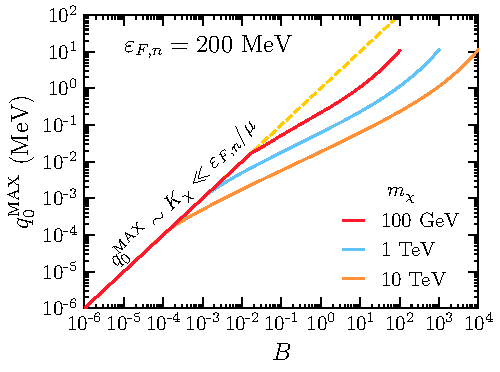
\includegraphics{q0max_Tdm.pdf}
  \caption{Maximum energy loss per collision with neutron targets, as a function of the DM kinetic energy. We have assumed $\kinFn=200\MeV$.} 
  \label{ch6:fig:q0max}
\end{figure}
%%%%%%%%%%%%%%%%%%%%%%%%%%%%%%%%%%%%%%%



In either regime, we can obtain first-order approximations for the average fraction of energy that a DM particle loses in a single collision by making use of the zero temperature approximation, a constant target mass, and nucleonic form factors at zero momentum transfer, i.e., $F(t)\sim1$. 
First, we consider the regime in which Pauli blocking is negligible, $m_\chi \gtrsim m_\chi^{\rm crit}$. For a constant cross-section (i.e. $\Msq \propto t^0$) we find 
\begin{equation}
  \langle \Delta K_\chi^{(n=0)} \rangle 
  \sim 2 \sqrt{\frac{\kinFi}{\mu}} K_\chi^{1/2} \ll K_\chi, 
\label{ch6:eq:aveElossn0largem}
\end{equation}
at first order in $m_\chi^{\rm crit}/m_\chi$. (See appendix 
% \ref{sec:pauliblockingle} for the corresponding approximation of the interaction rate, Eq.~\ref{ch6:eq:intraten0largem}.) 
~\fixMV{ADD APPENDIX} for the corresponding approximation of the interaction rate, Eq.~\fixMV{IN APPENDIX}) 
For cross-sections proportional to $t^1$ and $t^2$, the average energy losses
can be obtained in the same way, starting from the relevant expressions for  $\frac{d\Gamma}{d q_0}$.

Figure~\ref{ch6:fig:Taven0} shows the average energy loss fraction per collision. We see the  $\langle \Delta K_\chi^{(n=0)} \rangle/K_\chi \propto K_\chi^{-1/2}$ scaling of Eq.~\ref{ch6:eq:aveElossn0largem}
in the $m_\chi \gtrsim m_\chi^{\rm crit}$ phase of the evolution, where the kinetic energy is driven down toward values where Pauli blocking eventually becomes active. The latter Pauli blocked phase is indicated by the horizontal arrows in Fig.~\ref{ch6:fig:Taven0}. 





Moving to the case where Pauli blocking suppresses the scattering rate, $m_\chi\lesssim m_\chi^{\rm crit}$, the average energy loss per collision for the case of a constant cross-section is
\begin{equation}
\langle \Delta K_\chi^{(n=0)} \rangle \sim 
\frac{4}{7}K_\chi. 
\label{ch6:eq:aveElossn0}
\end{equation}
The average energy loss now scales linearly with $K_\chi$ (the flat regions in Fig.~\ref{ch6:fig:Taven0}) in contrast to the $K_\chi^{1/2}$ dependence of Eq.~\ref{ch6:eq:aveElossn0largem}.
As the DM kinetic energy decreases, the average fraction of energy transferred to the targets progressively increases until $K_\chi$ no longer satisfies Eq.~\ref{ch6:eq:mucrit} and consequently, the interaction rate becomes Pauli blocked.
As expected from Eq.~\ref{ch6:eq:mucrit}, the Pauli-suppressed region starts at higher kinetic energy for lower DM masses. 


%%%%%%%%%%%%%%%%%%%%%%%%%%%%%%%%%%%%%%%
\begin{figure}[t!bp]
  \centering
  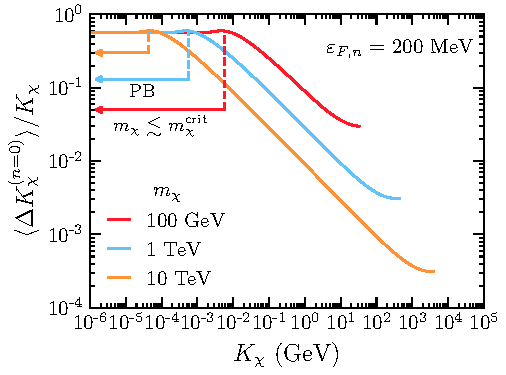
\includegraphics[width=0.495\textwidth]{q0ave_Tdm_n0.pdf}
  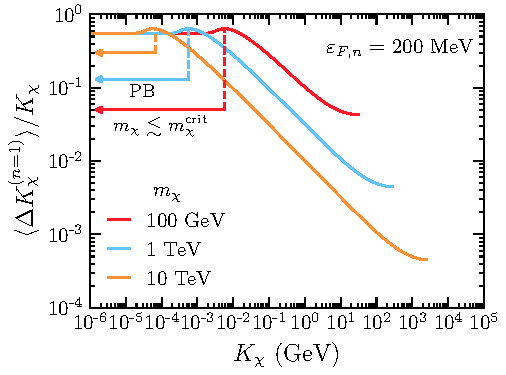
\includegraphics[width=0.495\textwidth]{q0ave_Tdm_n1.pdf}
  \caption{Average fraction of energy loss per DM-neutron collision for constant cross-section (left) and $d\sigma\propto t$ (right) as a function of the DM kinetic energy. Horizontal arrows indicate the Pauli blocked (PB) regime, $m_\chi\lesssim m_\chi^{\rm crit}$. 
  } 
  \label{ch6:fig:Taven0}
\end{figure}
%%%%%%%%%%%%%%%%%%%%%%%%%%%%%%%%%%%%%%%




For interactions with $t$-dependent matrix elements, the average energy loss per collision also scales linearly with $K_\chi$ in the Pauli blocked regime. For $\Msq \propto t^n$, with $n=1,2$, we find 
\begin{equation}
  \langle \Delta K_\chi^{(n=1)}\rangle \sim \frac{5}{9}K_\chi, \qquad 
  \langle \Delta K_\chi^{(n=2)} \rangle \sim \frac{28}{55}K_\chi ,
  \label{ch6:eq:aveElossn12}
\end{equation}
respectively, where we have used Eqs.~\fixMV{eq:intraten1} and \fixMV{eq:intraten2} for the interaction rates.
Note that the average energy loss fraction per collision exhibits similar behavior for all the interaction types considered,  
as seen by comparing the left and right panels of Fig.~\ref{ch6:fig:Taven0}. 
This is true in both the Pauli-blocked and non-blocked regimes.





%%%%%%%%%%%%%%%%%%%%%%%%%%%%%%%%%%%%%%%%%%%%%%%%%%%%%%%%%%%%%%%%%%%%%%%%%%%%%%%%%%%%
%%%%%%%%%%%%%%%%%%%%%%%%%%%%%%%%%%%%%%%%%%%%%%%%%%%%%%%%%%%%%%%%%%%%%%%%%%%%%%%%%%%%
\subsection{Thermalisation timescale}
\label{ch6:sec:thermstandard}
%%%%%%%%%%%%%%%%%%%%%%%%%%%%%%%%%%%%%%%%%%%%%%%%%%%%%%%%%%%%%%%%%%%%%%%%%%%%%%%%%%%%
%%%%%%%%%%%%%%%%%%%%%%%%%%%%%%%%%%%%%%%%%%%%%%%%%%%%%%%%%%%%%%%%%%%%%%%%%%%%%%%%%%%%




Once a DM particle is captured, it becomes gravitationally bound to the NS and follows an orbit that may or may not lie completely within the NS. If the orbit lies partly outside the NS, subsequent scatterings will be required for the DM particle to lose enough energy so that the complete orbit lies within the NS. This is the first stage in the thermalisation process. When estimating the amount of time needed for the DM orbit to lie completely within the star,  we find that this time is always much shorter than the full time required for DM to reach thermal equilibrium with the neutron targets. Consequently, this first step in the thermalisation process can be safely neglected. This finding is in agreement with Ref.~\cite{Garani:2018kkd_may_NewAnalysisNeutron}. 

We shall also assume that up-scattering of the DM to larger kinetic energy does not play an important role\footnote{Up-scattering refers to collisions with negative energy transfer $q_0<0$, such that the DM particle gains energy instead of losing it. When complete thermalisation has been achieved, the rates for up-scattering and down-scattering must become equal, and hence we expect the up-scattering rates to become more significant as thermalisation is approached.
If this were to be significant, our calculation below would underestimate the full thermalisation time. As we shall see, this does not impact our conclusions.}. These effects will become relevant as the DM approaches thermal equilibrium, increasing the thermalisation time. We estimate that up-scattering will, at most, increase the thermal equilibrium time by $\mathcal{O}(10\%)$, and thus we neglect this correction. 


For DM of mass much larger than the target mass, $m_\chi\gg \mbeff$, there is an additional stage in the thermalisation process where either Pauli blocking plays no role, or the interaction rate has a different power law relationship with the temperature than those identified in Section~\ref{sec:energyloss}. These initial scatterings make a negligible contribution to the thermalisation time, as  $\Gamma^{-}$ is a sharply decreasing function of the DM kinetic energy $K_\chi$. 

 
Let us denote the number of initial collisions before reaching the Pauli blocked regime as $N_1$, and the number of additional collisions required for complete thermalisation as $N_2$. For light DM, $m_\chi\lesssim \mbeff$, Pauli blocking affects the entire thermalisation process, i.e. $N_1=0$. Let $K_N$ be the kinetic energy after $N$ scatterings. After $N_1+N_2$ collisions, the DM will reach the equilibrium temperature $T_{\rm eq}$, which can be written as
\begin{equation}
K_{N_1+N_2} = 
K_{N_1}\left(1-\frac{\langle \Delta K_\chi \rangle}{K_\chi}\right)^{N_2} = \Tstareq,  
\label{ch6:eq:Teq}
\end{equation}
where we have used the fact that the average fractional energy loss is the same in each collision. 
The thermalisation time can then be defined as the sum of the average time between collisions, up until the final energy transfer is equal to $T_{\rm eq}$~\cite{Bertoni:2013bsa_dec_DarkMatterThermalization}
\begin{equation}
\tth = \sum_{n=0}^{N_2} \frac{1}{\Gamma^{-}(K_n)} \sim \sum_{n=N_1}^{N_2} \frac{1}{\Gamma^{-}(K_n)}.  
\label{ch6:eq:thermtime}
\end{equation}


For  $m_\chi \lesssim m_\chi^{\rm crit}$, the fraction of energy lost in the last few scatters is still a considerable fraction of the DM kinetic energy before the collision. Furthermore, these scatterings may take a considerably long time to occur, indicating that the process is discrete. 
As an example, consider thermalisation to a temperature of $10^3$~K, for a DM particle of mass $m_\chi=1\TeV$ and constant cross-section $\sigma_{n\chi} \sim 10^{-45}\cm^2$.\footnote{ For a wide DM mass range (GeV--TeV), this value is comparable to the cross-section that results in maximal capture, and hence we will use this cross-section as a reference value in some of the estimates that follow.} Hundreds of collisions are required to fully thermalise; the last 10 or so are spaced longer than a second apart; and the last couple are longer than $10 \kyr$ apart.    



To compute the thermalisation time, we numerically integrate Eq.~\ref{ch6:eq:diffGammaFiniteTemp} to obtain the interaction rate and the average energy lost in each collision for each of the EFT operators in Table~\ref{ch6:tab:opers_defn_full}. We find that the thermalisation time for a particular interaction type scales according to the dominant power of the Mandelstam variable $t$ in the corresponding matrix element; see the last column of  Table~\ref{ch6:tab:opers_defn_full}. Thus, to understand how the thermalisation times scale, it is enough to consider differential cross-sections that are proportional to a given power of $t$, i.e. $d\sigma\propto t^n$, with $n=0,1,2$. 
Below, we present results for operators that depend only on $t$ (D1-4 in Table~\ref{ch6:tab:opers_defn_full}), and not on the centre of mass energy, $s$. In Appendix~\fixMV{Add s dep appendix}, we outline the procedure used to obtain analytic expressions for those operators with an explicit dependence on $s$ (operators D5-10). 


In Figure~\ref{ch6:fig:thermtime}, we show the full numerical results for the thermalisation time as a function of the DM mass for different equilibrium temperatures. It is clear that the power law scaling of the thermalisation time with DM mass depends on whether $m_\chi$ is larger or smaller than the nucleon mass. To understand these results, we make use of the analytic approximations for the average DM energy loss derived in Section~\ref{sec:energyloss} and valid in the zero temperature limit. 

%%%%%%%%%%%%%%%%%%%%%%%%%%%%%%%%%%%%
\begin{figure}[t!bp]
\centering 
  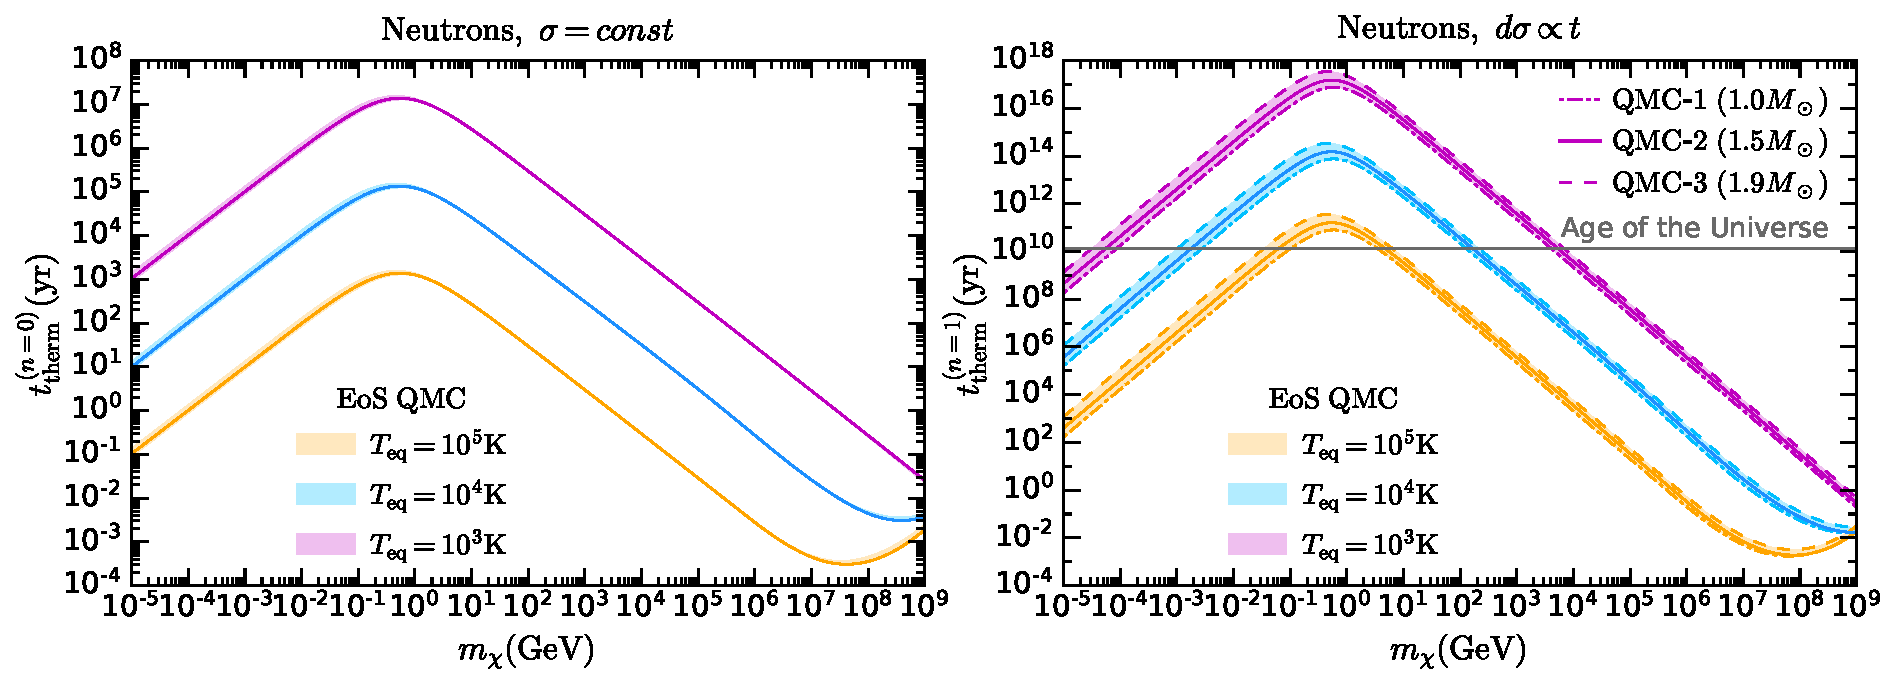
\includegraphics[width=\textwidth]{ttherm_mdm_n0_n1.pdf}
  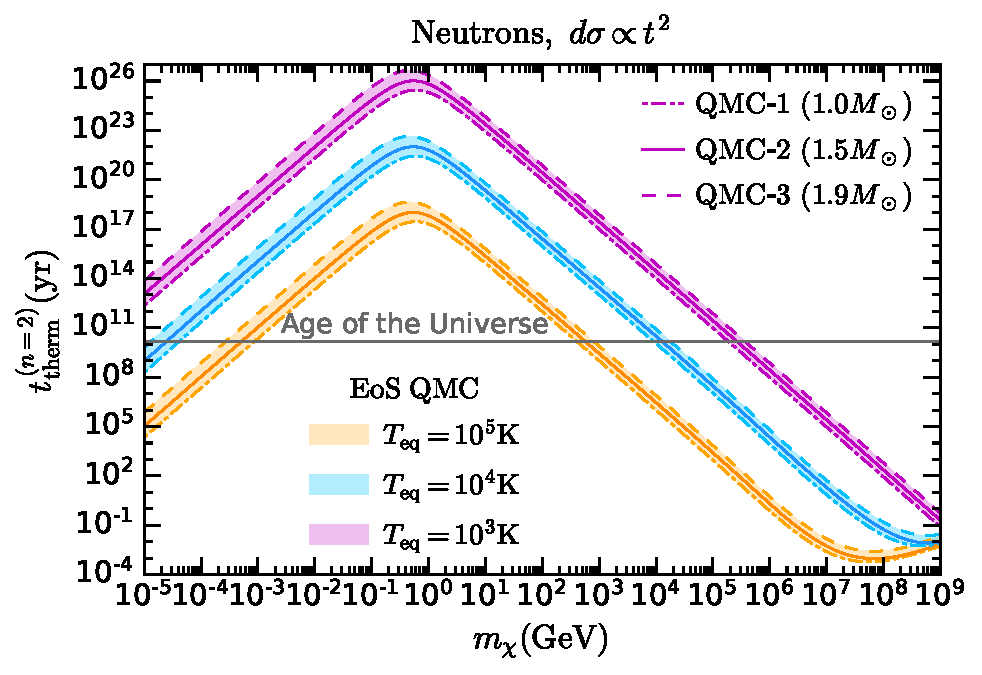
\includegraphics[width=.525\textwidth]{ttherm_n2_eos.pdf}
  \caption{thermalisation time as a function of the DM mass for constant cross-section (top left), $d\sigma \propto t$ (top right)  and $d\sigma\propto t^2$ (bottom). We have used the NS benchmark models in Table~\ref{ch6:tab:QMC_configs} and a reference cross-section of $\sigma_{\rm n\chi}= 10^{-45}\cm^2$ close to the NS surface. Shaded regions indicate the variation with the choice of EoS: QMC-1 (dot-dashed), QMC-2 (solid), and QMC-3 (dashed). 
  }
  \label{ch6:fig:thermtime}
\end{figure}
%%%%%%%%%%%%%%%%%%%%%%%%%%%%%%%%%%%%


We begin by studying the Pauli blocked regime, $m_\chi \lesssim m_\chi^{\rm crit}$. 
In this case, the majority of the thermalisation time is dictated by the final few scatters, for which the form factors are close to their value at zero momentum transfer.  These last collisions occur close to the NS centre, so we can take the target mass as constant and equal to the value at the centre of the star, $\mbeff(0)$. For the case of a constant DM-neutron cross-section, $d\sigma \propto t^0$, the thermalisation time can thus be obtained by using  Eqs.~\fixMV{eq:intraten0}, \ref{ch6:eq:Teq} and \ref{ch6:eq:aveElossn0} in Eq.~\ref{ch6:eq:thermtime}. This leads to
%
\footnotesize
\begin{equation}
  \tthn{0} \sim   \frac{147}{16 }\frac{\pi^2 m_\chi}{ \left(\mbeff(0) + m_\chi\right)^2}\frac{1}{\sigma_{i\chi}^{n=0}}\frac{1}{T_{\rm eq}^2}, 
  \label{ch6:eq:thermtimen0}
\end{equation} 
\normalsize
%
where $\sigma_{i\chi}^{n=0}$ is the DM-baryon cross-section. 
The scaling of this expression with $\Tstareq$, DM mass, and DM-target cross-sections 
agrees with Ref.~\cite{Bertoni:2013bsa_dec_DarkMatterThermalization}. 
Numerically we obtain
\footnotesize
\begin{equation}
  \tthn{0} \sim \begin{dcases}
    4.4\times 10^{6}\yrs \, \left(\frac{m_\chi}{10\MeV}\right)\left(\frac{10^{-45}\cm^2}{\sigma_{i\chi}^{n=0}}\right)\left(\frac{10^3K}{T_{\rm eq}}\right)^{2},\quad m_\chi \ll \mbeff(0)\\
    9.7\times 10^{6}\yrs \, \left(\frac{10\GeV}{m_\chi}\right)\left(\frac{10^{-45}\cm^2}{\sigma_{i\chi}^{n=0}}\right)\left(\frac{10^3K}{T_{\rm eq}}\right)^{2},\quad m_\chi \gg \mbeff(0)
  \end{dcases} \label{ch6:eq:t_therm_0}
\end{equation}
\normalsize
%
where we have set $\mbeff(0) = 0.5\,m_n$. 
The $m_\chi$ dependence of these expressions explains the features observed in the top left panel of Fig.~\ref{ch6:fig:thermtime}. For $m_\chi \ll \mneff(0)$, the thermalisation time scales with the DM mass as the number of scatterings needed for thermalisation increases. Conversely, for $m_\chi \gg \mneff(0)$, $\tthn{0}$ is inversely proportional to $m_\chi$ due to the reduced Pauli blocking, explaining the change of slope around the value of the neutron effective mass in the NS centre. 




We repeat the same analysis for cross-section proportional to higher powers of $t$, i.e., $d\sigma \propto t^n$ with $n=1,2$. Using Eqs.~\fixMV{eq:intraten1}, \fixMV{eq:intraten2} and \ref{ch6:eq:aveElossn12}, we find
% 
\small
\begin{align}
    \tthn{1} &\sim 14 %\frac{2187}{152}
    \frac{\pi^2 m_\chi^2 (\mbeff(0))^2}{\left(\mbeff(0) + m_\chi\right)^2 \left((\mbeff(0))^2+ m_\chi^2\right)}\frac{1}{\sigma_{i\chi}^{n=1}}\frac{1}{T_{\rm eq}^3} \frac{1-B(\Rstar)}{B(\Rstar)},  
    \label{ch6:eq:thermtimen1}\\
    \tthn{2} &\sim 17 %\frac{27451875}{1231312}
    \frac{\pi^2 m_\chi^3 (\mbeff(0))^4}{\left(\mbeff(0) + m_\chi\right)^2 \left((\mbeff(0))^2+ m_\chi^2\right)^2}\frac{1}{\sigma_{i\chi}^{n=2}}\frac{1}{T_{\rm eq}^4} \left[\frac{1-B(\Rstar)}{B(\Rstar)}\right]^2, 
    \label{ch6:eq:thermtimen2}
\end{align}
\normalsize
% 
where the factors involving $B(R_\star)$ arise from fixing the cross-section to its value at the surface; 
see Appendix~\fixMV{sec:pauliblockingle} for details.


To gain insight into the order of magnitude of these thermalisation times, we set  $B(\Rstar)=0.5$ and $\mbeff(0) = 0.5\,m_n$, yielding
% 
\footnotesize{
\begin{align}
    \tthn{1} &\sim \begin{dcases}
        2.5\times 10^{14}\yrs \, \left(\frac{m_\chi}{10\MeV}\right)^2\left(\frac{10^{-45}\cm^2}{\sigma_{i\chi}^{n=1}}\right)\left(\frac{10^3K}{T_{\rm eq}}\right)^{3},\quad m_\chi \ll \mbeff(0)\\
        3.9\times 10^{15}\yrs \, \left(\frac{10\GeV}{m_\chi}\right)^2\left(\frac{10^{-45}\cm^2}{\sigma_{i\chi}^{n=1}}\right)\left(\frac{10^3K}{T_{\rm eq}}\right)^{3},\quad m_\chi \gg \mbeff(0)
    \end{dcases}
    \label{ch6:eq:t_therm_1} \\
   \tthn{2} &\sim\begin{dcases}
        1.1\times 10^{23}\yrs \, \left(\frac{m_\chi}{10\MeV}\right)^3\left(\frac{10^{-45}\cm^2}{\sigma_{i\chi}^{n=2}}\right)\left(\frac{10^3K}{T_{\rm eq}}\right)^{4},\quad m_\chi \ll \mbeff(0)\\
        1.2\times 10^{24}\yrs \, \left(\frac{10\GeV}{m_\chi}\right)^3\left(\frac{10^{-45}\cm^2}{\sigma_{i\chi}^{n=2}}\right)\left(\frac{10^3K}{T_{\rm eq}}\right)^{4},\quad m_\chi \gg \mbeff(0).
    \end{dcases}
    \label{ch6:eq:t_therm_2}
\end{align} 
}
\normalsize
% 
As anticipated, we see that the momentum-suppressed cross-sections translate into significantly longer thermalisation times than for the case of a constant (unsuppressed) cross-section.
These expressions also allow us to understand the dependence of $\tth$ on the DM mass.
For $d\sigma\propto t^n$, the thermalisation time scales as $m_\chi^{n+1}$ for $m_\chi \ll \mneff(0)$, and as the inverse of this quantity for $m_\chi \gg \mneff(0)$.



The choice of EoS has a small but non-negligible impact on the thermalisation time, as indicated by the widths of the shaded regions in Fig.~\ref{ch6:fig:thermtime}. 
For a constant cross-section, we observe almost no variation in $\tth$ with the NS configuration, except for the $m_\chi \lesssim m_n$ region. This is due to the dependence of $\mneff(0)$ on the NS model; see Table~\ref{ch6:tab:QMC_configs} and Eq.~\ref{ch6:eq:thermtimen0}.
For cross-sections $d\sigma\propto t^n$, with $n=1,2$, the dependence on $B(\Rstar)$ in Eqs.~\ref{ch6:eq:thermtimen1} and \ref{ch6:eq:thermtimen2} adds an extra dependence on the choice of NS model. For these momentum-suppressed interactions, DM requires more time to reach an equilibrium temperature in heavier NSs. This is due to the combination of two effects: the effective mass of the targets in the centre of the NS is smaller in more massive NS configurations, while $B(\Rstar)$ increases. Nonetheless, the dependence on NS configuration remains relatively mild. 

%%%%%%%%%%%%%%%%%%%%%%%%%%%%%%%%%%%%%



We now turn to the $m_\chi \gtrsim \mcrit$ regime, which is observed only for temperatures above $10^4\K$ in Fig.~\ref{ch6:fig:thermtime}. This regime change is indicated by the change of slope that occurs at large DM masses, clearly evident for  $T_{eq}=10^5\K$ (orange)  at a DM of mass $m_\chi\gtrsim5\times10^7\GeV$.  
In this regime, the energy lost in each collision is a tiny fraction of the initial DM kinetic energy, and the time between scatterings is of order a fraction of a second. This indicates that a continuous approximation becomes more appropriate than a discrete sum to estimate $\tth$.
In this case, the momentum-dependent part of the form factor, $F(t)$, will be relevant only at the beginning of the thermalisation process and become less and less relevant as the average momentum transfer decreases in each subsequent scatter.\footnote{We have numerically verified that the $t$-dependent form factors do not alter the results in any significant manner.} It is these low momentum-transfer collisions that dominate the thermalisation time.
%
For a constant cross-section ($n=0$), in the zero temperature approximation, we obtain 
(see Appendix~\fixMV{sec:thermsuperheavy} for details)
\begin{equation}
    \tthn{0} \sim \frac{9 \pi^2 m_\chi}{8 (\mbeff(0))^2 \kinFi^2 \sigma_{i\chi}^{n=0} }\log\left[\frac{m_\chi}{T_{\rm eq}}\left(\frac{1}{\sqrt{B(\Rstar)}}-1\right)\right]. %\quad m_\chi\gtrsim m_\chi^{\rm crit}.
\label{ch6:eq:tthemheavy0text}
\end{equation}
In this super heavy DM mass regime, we see that the thermalisation time is an increasing function of $m_\chi$. 


It is worth remarking that for a constant DM-neutron cross-section (top left panel) thermalisation will always occur within the age of the Universe. However, this is not true for momentum-suppressed cross-sections, for a range of DM masses. Specifically, for $T_{\rm eq}=10^3\K$ and the assumed reference cross-section,  DM of mass $m_\chi\lesssim 10 \TeV$ ($m_\chi\lesssim 1 \PeV$)  will not have enough time to  thermalise  for $d\sigma \propto t$ ($d\sigma \propto t^2$).
Importantly, however, we shall see below that even when full thermalisation takes longer than the age of the Universe, the majority of the kinetic energy is deposited on a much shorter timescale.



Finally, we must incorporate the fact that DM will scatter with various baryonic species in the NS rather than just the neutrons. To do this, the thermalisation times from scattering off each species are combined appropriately based on their abundances. Specifically, we sum the inverse single-species thermalisation times, weighted by their relative abundance at the centre of the NS, such that
\begin{equation}
    \frac{1}{t_{\text{therm},\; \text{tot}}} = \sum_i \frac{Y_i(0)}{t_{\text{therm},\;i}},
    \label{ch6:eq:tthermtot}
\end{equation}
where $Y_i(0)$ is the abundance of the species in the centre of the NS, and the sum runs over all possible baryons. For the case of the heaviest NS we consider, 1.9 $\Msun$, this includes the $\Lambda^0$, $\Xi^0$ and $\Xi^-$ hyperons. The resulting thermalisation time then lies between the fastest and slowest single-species times, as is expected.










%%%%%%%%%%%%%%%%%%%%%%%%%%%%%%%%%%%%%%%%%%%%%%%%%%%%%%%%%%%%%%%%%%%%%%%%%%%%%%%%%%%%
%%%%%%%%%%%%%%%%%%%%%%%%%%%%%%%%%%%%%%%%%%%%%%%%%%%%%%%%%%%%%%%%%%%%%%%%%%%%%%%%%%%%
\section{Capture-Annihilation Equilibrium}
\label{ch6:sec:CAEquilibrium}
%%%%%%%%%%%%%%%%%%%%%%%%%%%%%%%%%%%%%%%%%%%%%%%%%%%%%%%%%%%%%%%%%%%%%%%%%%%%%%%%%%%%
%%%%%%%%%%%%%%%%%%%%%%%%%%%%%%%%%%%%%%%%%%%%%%%%%%%%%%%%%%%%%%%%%%%%%%%%%%%%%%%%%%%%




The captured DM will accumulate in the centre of the NS, where it will begin to annihilate. The annihilation rate will grow until sufficient time has elapsed for the capture and annihilation processes to reach equilibrium. In this limit, the total amount of DM in the NS is maximised and will remain constant. Once this occurs, annihilation efficiently deposits the DM mass-energy into the star. 


Let us begin by assuming that the dark matter has fully thermalised. After reviewing the standard capture-annihilation equilibrium calculation, we will relax this assumption to consider the more general case of partially thermalised dark matter and derive new expressions that hold in that scenario. Importantly, we shall see that capture-annihilation equilibrium, and hence efficient annihilation can occur without full thermalisation.

%%%%%%%%%%%%%%%%%%%%%%%%%%%%%%%%%%%%%%
\subsection{Capture-annihilation equilibrium of thermalised dark matter}
%%%%%%%%%%%%%%%%%%%%%%%%%%%%%%%%%%%%%%


The thermalised DM will collect within an isothermal sphere at the centre of the NS where it will begin to annihilate. The efficiency of the annihilation will depend on the volume of this sphere, which is expected to be very small for the DM masses we consider. 
Very close to the centre of the NS, the density does not vary significantly and can be taken to be constant. Then, working in the weak field approximation such that $B(r) \sim  1+2\Phi(r)$, 
we can obtain the gravitational potential inside the NS,
\begin{align}
\Phi(r) & = -\int_r^\infty \frac{G M_\star(r')}{r'^2}dr' 
\approx \frac{2}{3}\pi G \rho_c r^2, 
\end{align}
where $\rho_c$ is the central density of the NS. 
The  number density of DM particles that have thermalised to a temperature $\Tstareq$ as a function of radius will then be given by a Maxwell-Boltzmann distribution
\begin{align}
n_{\chi}(r) & \simeq n_0 \exp\left[ -\frac{m_\chi\Phi(r)}{T_{\rm eq}}\right] 
= \frac{N_\chi}{\pi^{3/2}  r_{\rm iso}^3}\exp\left( -\frac{r^2}{ r_{\rm iso}^2}\right), 
\end{align}
where $N_\chi$ is the total number of DM particles within the isothermal sphere, and $r_{\rm iso}$ is the radius of the DM isothermal sphere. 
Applying the viral theorem leads to the following expression for $r_{\rm iso}$, 
\begin{align}
r_{\rm iso} & = \sqrt{\frac{3 \Tstareq}{2\pi G m_\chi \rho_c}} \nonumber\\
& \approx  0.26\,\text{m}\left[\left(\frac{T_{\rm eq}}{10^3\,\text{K}}\right)\left(\frac{1\GeV}{m_\chi}\right)\left(\frac{8\times10^{14}\,\textrm{g}\,\text{cm}^{-3}}{\rho_c}\right)\right]^{1/2}.
\end{align}
The total number of DM particles enclosed in this sphere is then
\begin{equation}
    N_\chi    \simeq  4\pi\int dr \, r^2n_{\chi}(r),
\end{equation} 
and the velocity distribution of the thermalised DM is  given by
\begin{equation}
f_{\rm MB}(v_\chi)  = 4\pi \left(\frac{m_\chi}{4 \pi \Tstareq}\right)^{3/2} v_\chi^2 \exp\left[ -\frac{m_\chi v_\chi^2}{4 \Tstareq} \right].
\end{equation}




In the absence of evaporation, which can safely be neglected for $m_\chi \gtrsim 1.17\times 10^{-8}\GeV$ for a Gyr old NS with core temperature $\sim 10^3\K$~\cite{Bell:2020lmm_mar_ImprovedTreatmentDark}, the time evolution of the total number of DM particles present inside the NS is governed by
\begin{equation}
    \frac{dN_\chi}{dt} = C - A N_\chi^2 \label{ch6:eq:ndm}.
\end{equation}
Here $C$ is the capture rate and  $A$ is related to the DM annihilation rate, $\Gamma_{\rm ann}$, through
\begin{equation}
    \Gamma_{\rm ann} =  \frac{1}{2}A N_\chi^2,
\end{equation}
where
\begin{equation}
    A = \frac{\langle \sigma_\text{ann}v_\chi \rangle}{N_\chi^2} \int n_\chi^2(r) d^3 r \simeq \frac{\langle \sigma_\text{ann} v_\chi\rangle}{(2\pi)^{3/2} r_{\rm iso}^3}, \label{ch6:eq:annrate}
\end{equation}
and $\langle \sigma_{\rm ann} v_\chi \rangle$ is the
thermally averaged DM annihilation cross-section. These are given in Table~\ref{ch6:tab:annCS} for the EFT interactions we consider, where $\langle v^2_\chi \rangle = v_{\rm th}^2 =  6 \Tstareq/ m_\chi$.


We note that the cross-sections shown in Table~\ref{ch6:tab:annCS} are quark-level expressions. For most of the mass range of interest, these provide excellent approximations to the hadron-level annihilation cross-sections, provided we impose a lower bound on the DM mass for which an annihilation channel is open, taken to be the pion mass. See Appendix~\fixMV{sec:quarkhadron} for details.




%%%%%%%%%%%%%%%%%%%%%%%%%%%%%%%%%%%%%%%%%%%%%%%%%%%%%%%%%%%%%%%%
\begin{table}[t]
    \centering
    \begin{tabular}{c c l}
    \toprule
         Name & Operator & $\langle \sigma_{ann} v_\chi\rangle$\\
        \midrule\midrule 
         D1  & $\bar\chi  \chi\;\bar q  q $ & 
         $\frac{3 m_\chi^2}{8\pi\Lambda^4}\sum_q y_q^2 \left( 1 - \frac{m_q^2}{m_\chi^2}\right)^{3/2} v_{\rm th}^2 $\\ 
         D2  &  $\bar\chi \gamma^5 \chi\;\bar q q $ & \small $\frac{3 m_\chi^2}{2\pi \Lambda^4}\sum_q y_q^2 \sqrt{1 - \frac{m_q^2}{m_\chi^2}} \left[ \left( 1 - \frac{m_q^2}{m_\chi^2}\right) + \frac{3}{8}\frac{m_q^2}{m_\chi^2}v_{\rm th}^2\right]$\\
         D3  & $\bar\chi \chi\;\bar q \gamma^5  q $  & \small $\frac{3 m_\chi^2}{8\pi\Lambda^4}\sum_q y_q^2 \sqrt{ 1 - \frac{m_q^2}{m_\chi^2}} v_{\rm th}^2$\\
         D4  & $\bar\chi \gamma^5 \chi\; \bar q \gamma^5 q $ & \small $ \frac{3 m_\chi^2}{2\pi\Lambda^4}\sum_q y_q^2 \sqrt{1 - \frac{m_q^2}{m_\chi^2}}\left[ 1 + \frac{m_q^2}{8(m_\chi^2 - m_q^2)} v_{\rm th}^2\right]$\\
         D5  & $\bar \chi \gamma_\mu \chi\; \bar q \gamma^\mu q$ & \small $\frac{3 m_\chi^2}{2\pi \Lambda^4}\sum_q \sqrt{1 - \frac{m_q^2}{m_\chi^2}} \left[ \left( 2 +\frac{m_q^2}{m_\chi^2}\right) + \left( \frac{-4m_\chi^4 +2m_q^2 m_\chi^2 +11m_q^4}{24m_\chi^2 ( m_\chi^2 - m_q^2)} \right) v_{\rm th}^2 \right]$\\
         D6  & $\bar\chi \gamma_\mu \gamma^5 \chi\; \bar  q \gamma^\mu q $ & \small $\frac{m_\chi^2}{4\pi \Lambda^4}\sum_q \sqrt{1 - \frac{m_q^2}{m_\chi^2}} \left[ 2 +\frac{m_q^2}{m_\chi^2}\right] v_{\rm th}^2$\\
         D7  & $\bar \chi \gamma_\mu  \chi\; \bar q \gamma^\mu\gamma^5  q$  & \small $ \frac{3 m_\chi^2 }{\pi\Lambda^4}\sum_q \sqrt{1 - \frac{m_q^2}{m_\chi^2}} \left[ \left( 1 - \frac{m_q^2}{m_\chi^2} \right) - \frac{1}{24}\left( 2 - 11\frac{m_q^2}{m_\chi^2}\right) v_{\rm th}^2 \right]$ \\
         D8  & $\bar \chi \gamma_\mu \gamma^5 \chi\; \bar q \gamma^\mu \gamma^5 q $ & \small $ \frac{3 m_\chi^2}{2\pi \Lambda^4} \sum_q \sqrt{1 - \frac{m_q^2}{m_\chi^2}} \left[ \frac{m_q^2}{m_\chi^2} + \left( \frac{8m_\chi^4 - 28m_\chi^2 m_q^2 + 23 m_q^4}{24 m_\chi^2(m_\chi^2 - m_q^2)} \right) v_{\rm th}^2 \right] $ \\
         D9  & $\bar \chi \sigma_{\mu\nu} \chi\; \bar q \sigma^{\mu\nu} q $  & \small $ \frac{6 m_\chi^2}{\pi\Lambda^4} \sum_q \sqrt{1 - \frac{m_q^2}{m_\chi^2}} \left[ \left( 1 + 
         2\frac{m_q^2}{m_\chi^2}\right) -\left( \frac{2m_\chi^4 +17m_q^2 m_\chi^2 -28m_q^4}{24m_\chi^2(m_\chi^2 - m_q^2) }\right) v_{\rm th}^2\right] $ \\     
         D10 & $\bar \chi \sigma_{\mu\nu} \gamma^5\chi\; \bar q \sigma^{\mu\nu} q$ & \small $\frac{6 m_\chi^2}{\pi\Lambda^4} \sum_q \sqrt{1 - \frac{m_q^2}{m_\chi^2}} \left[ \left( 1 - \frac{m_q^2}{m_\chi^2}\right)  -\frac{1}{24}\left(2 -17\frac{m_q^2}{m_\chi^2}\right) v_{\rm th}^2 \right] $\\
         \bottomrule
    \end{tabular}
    \caption{Thermally averaged annihilation cross-sections $\sigmav$ for the dimension 6 EFT operators, expanded to second order in $v_\chi$. The $y_q$ factors are the quark Yukawa couplings~\cite{Zheng:2010js_Constraininginteractionstrength}.}
    \label{ch6:tab:annCS} 
\end{table}
%%%%%%%%%%%%%%%%%%%%%%%%%%%%%%%%%%%%%%%%%%%%%%%%%%%%%%%%%%%%%%%%




The solution to Eq.~\ref{ch6:eq:ndm} in terms of the capture and annihilation rates is
%
\begin{equation}
    N_\chi(t) = \sqrt{\frac{C}{A}}\tanh\left(\sqrt{CA} \,t\right).\label{ch6:eq:Noft}
\end{equation}
%
Ultimately, we are interested in the behavior of Eq.~\ref{ch6:eq:Noft} at late stages in the NS evolution, i.e., for $t\rightarrow \tstar$, where $\tstar$ is the age of the NS, which we take to be $\sim 1\Gyr$. In this limit, the hydrostatic NS structure, and hence the capture rate, are not expected to change with time. Of particular interest is whether or not an equilibrium is reached between the capture and annihilation rates. Such a state is reached for timescales greater than 
\begin{equation}
     t_{\rm eq} = \frac{1}{\sqrt{C A}}.
     \label{ch6:eq:teqold}
\end{equation}
For earlier times, $ t < t_{\rm eq}$, one can neglect the loss of DM particles due to annihilation, leaving $N_\chi\sim C t$. 


%%%%%%%%%%%%%%%%%%%%%%%%%%%%%%%%%%%%%%
\subsection{Capture-annihilation equilibrium of partially\\ thermalised dark matter}
%%%%%%%%%%%%%%%%%%%%%%%%%%%%%%%%%%%%%%



The standard calculation of the annihilation rate, using Eq.~\ref{ch6:eq:annrate}, assumes that the DM has thermalised, i.e., $t > t_{\rm therm}$. 
If thermalisation has not been achieved by a time $t\sim\tstar<\tth$, the DM kinetic energy distribution will peak around the lowest temperature that DM has had enough time to reach. This is given by 
%
\begin{equation}
K_\chi \sim T_{\rm eq} \left(\frac{\tth+\tstar}{\tstar}\right)^{\frac{1}{2+n}},
\label{ch6:eq:lowtemp} 
\end{equation}
%
where $n$ is the exponent of the dominant $t^n$ term in the differential cross-section, $d\sigma \propto t^n$, as given in the last column of Table~\ref{ch1:tab:opers_defn_full}. See Appendix~\fixMV{sec:minTempDerivation} for details. 
We can then find the radius of the DM distribution (which is no longer isothermal) and the $\sigmav$ corresponding to the peak of the energy distribution $K_\chi$. 
We obtain $A$ via the replacement  
%
\begin{equation}
    A \rightarrow A \left(\frac{T_\text{eq}}{K_\chi}\right)^{\alpha} = 
   A \left(\frac{\tstar}{t_\text{therm}+\tstar}\right)^{\frac{\alpha}{2+n}},  
\end{equation}
%
where $\alpha=3/2$ for $s$-wave annihilation, and $\alpha=1/2$ for $p$-wave. 
Making this replacement in Eq.~\ref{ch6:eq:teqold} leads to a capture-annihilation equilibrium time of
\begin{equation}
 t_{\rm eq} = \frac{1}{\sqrt{C A}} \left(\frac{t_\text{therm}+\tstar}{\tstar}\right)^{\frac{\alpha}{2(2+n)}}. \label{ch6:eq:teq} 
\end{equation}

No previous estimate of the capture-annihilation equilibrium time has considered the case of partially thermalised DM. If thermalisation has not been achieved, the additional factor in Eq.~\ref{ch6:eq:teq}, compared to Eq.~\ref{ch6:eq:teqold}, increases the equilibrium time. (Or, equivalently, increases the cross-sections required to reach equilibrium within a specified time.) However, it is critical to realize that $t_\text{eq}$ can be shorter than $t_\text{therm}$. 
In fact, annihilation can occur efficiently even if complete thermalisation never occurs. In this scenario, we must use Eq.~\ref{ch6:eq:teq}.



Assuming the DM is captured at the geometric limit, we arrive at the following result for our benchmark NS QMC-2
\begin{eqnarray}
    t_{\rm eq}  &\sim&  4\times10^{-6}\yr\left(\frac{100\GeV}{m_\chi}\right)^{\frac{1}{4}}\left(\frac{10^{-26}\cm^3 \s^{-1}}{\langle\sigma_\text{ann} v_\chi\rangle}\right)^{\frac{1}{2}} \left(\frac{1\GeV\cm^{-3}}{\rho_\chi}\right)^{\frac{1}{2}}\left(\frac{T_{\rm eq}}{10^3\K}\right)^{\frac{3}{4}} 
    \nonumber \\ &&\times
    \left(\frac{t_{\rm therm}+\tstar}{\tstar}\right)^{\frac{\alpha}{2(2+n)}}.
\end{eqnarray}
Comparing this expression with the thermalisation times in the previous section, we anticipate that  $t_\text{eq}$ will typically be shorter than $t_\text{therm}$, often by many orders of magnitude.




%%%%%%%%%%%%%%%%%%%%%%%%%%%%%%%%%%%%%%%%%%%%%%%%
%%%%%%%%%%%%%%%%%%%%%%%%%%%%%%%%%%%%%%%%%%%%%%%%
\section{Neutron Star Heating Timescales}
\label{ch6:sec:results}
%%%%%%%%%%%%%%%%%%%%%%%%%%%%%%%%%%%%%%%%%%%%%%%%
%%%%%%%%%%%%%%%%%%%%%%%%%%%%%%%%%%%%%%%%%%%%%%%%



%%%%%%%%%%%%%%%%%%%%%%%%%%%%%%%%%%%%%%%%%%%%%%%%
\subsection{Kinetic heating timescale}
\label{ch6:subsec:KinHeating}
%%%%%%%%%%%%%%%%%%%%%%%%%%%%%%%%%%%%%%%%%%%%%%%%


It has commonly been assumed that the DM kinetic energy deposition occurs instantaneously. However, it is not immediately obvious that this is true. In particular, for scattering interactions suppressed by powers of the momentum transfer, $t$, full thermalisation can take longer than the age of the Universe. We must therefore determine whether a {\it significant fraction} of the initial kinetic energy can be deposited on a shorter timescale.



To quantify the timescale on which kinetic heating takes place, we define $t_{\rm kin}$ to be the time required for a DM particle to lose 99\% of its maximum kinetic energy, $K_\chi = m_\chi (1/\sqrt{B(0)} - 1)$.  
This time is calculated in the same way as the thermalisation time, while also keeping track of the time the DM spends outside the star along its orbit, i.e., the initial stage of the thermalisation process that was neglected in Section~\ref{sec:thermstandard}. For simplicity, the DM particle orbits are taken to be linear, passing through the centre of the star, with the radial extent calculated using the geodesic equations. We expect an ${\cal O}(1)$ correction to our results when considering circular orbits.
Additionally, we randomize the radial position in the NS where the DM interacts with a target. 

%%%%%%%%%%%%%%%%%%%%%%%
\begin{figure}[t!bp]
    \centering  
    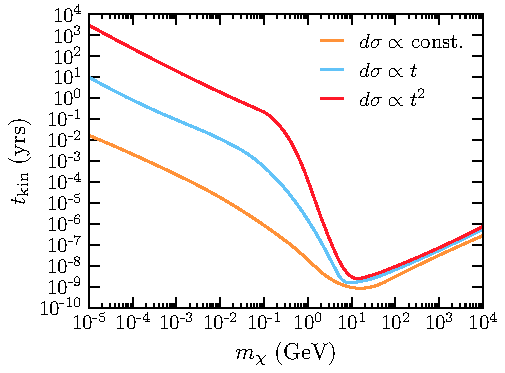
\includegraphics{kinheattime_mdm.pdf}
    \caption{Timescale on which the DM deposits $99\%$ of its initial kinetic energy in the NS. We have assumed an NS with configuration QMC-2, and a DM-neutron scattering cross-section of $\sigma_{n\chi}=10^{-45}\cm^2$ at the surface of the star. 
    }
    \label{ch6:fig:kinheattimes}
\end{figure}
%%%%%%%%%%%%%%%%%%%%%%%

Figure~\ref{ch6:fig:kinheattimes} shows the time required for kinetic heating to be achieved, assuming DM-neutron interactions of the form $d\sigma \propto t^n$, with cross-sections normalized to $\sigma_{n\chi} = 10^{-45}\cm^2$ at the surface of the star. As the location of each interaction is randomized, these results are obtained by averaging over several simulations for each DM mass. For light DM, $t_{\rm kin}$ decreases with increasing DM mass, due to the decreased effects of Pauli blocking, with the change of slope at $m_\chi \sim 0.1\GeV$ indicating the point where Pauli blocking affects only a fraction of the total process.
For masses $\gtrsim 10\GeV$, Pauli blocking is not relevant to this part of the thermalisation process, and hence the $t_{\rm kin}$ monotonically increases with the DM mass, as was seen in the thermalisation of super-heavy DM. 

Fig.~\ref{ch6:fig:kinheattimes} illustrates two key facts. First, $t_{\rm kin}$ differs by orders of magnitude for the different cross-section types, $d\sigma\propto t^n$, with larger values of $t_{\rm kin}$ for the most highly momentum-suppressed interactions, as expected. Second, and importantly, the kinetic heating occurs relatively quickly for all interaction types, on timescales much shorter than a typical NS age. Indeed, for the case of a constant cross-section, $\tkin$ is much shorter than a year.



%%%%%%%%%%%%%%%%%%%%%%%%%%%%%%%%%%%%%%%%%%%%%%%%
\subsection{Annihilation heating timescale}
\label{ch6:subsec:AnnHeatTimes}
%%%%%%%%%%%%%%%%%%%%%%%%%%%%%%%%%%%%%%%%%%%%%%%%



%%%%%%%%%%%%%%%%%%%%%%%%%%
\begin{figure}[t!bp]
\centering    
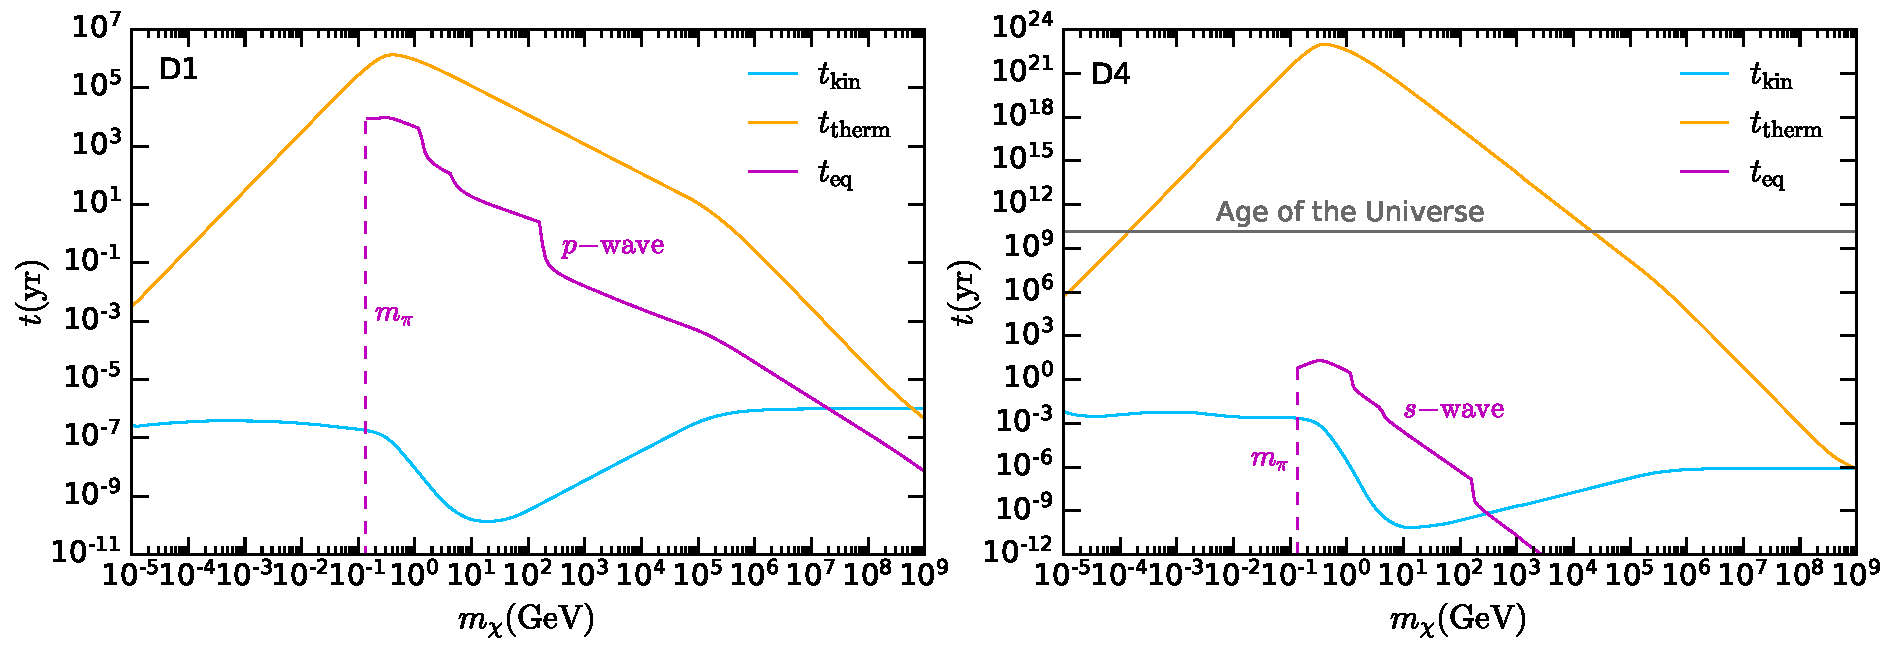
\includegraphics[width=\textwidth]{timescales_maxcap_n.pdf}
    \caption{Timescales for kinetic heating (blue), thermalisation (orange), and capture-annihilation equilibrium (magenta), for operators D1 (left) and D4 (right). The operator D1 has an unsuppressed scattering cross-section and a $p$-wave suppressed annihilation cross-section, while $D4$ has a $q_\text{tr}^4$ suppressed scattering cross-section and an unsuppressed ($s$-wave) annihilation cross-section.
    The interaction strength has been chosen to give maximal capture. (Specifically, we used $\Lambda_q$ values corresponding to a capture cross-section at the geometric limit, assuming scattering with the neutron targets in the QMC-2 NS.)   
    }
    \label{ch6:fig:timescales}
\end{figure}
%%%%%%%%%%%%%%%%%%%%%%%%%%



Figure~\ref{ch6:fig:timescales} shows all relevant timescales for DM-induced heating of old neutron stars. These timescales have been calculated considering DM scattering off the neutron targets in the benchmark NS QMC-2, for the case of maximal capture, $f = 1$ (i.e., we have set the EFT parameter $\Lambda_q$ as required to achieve capture at the geometric limit).
We show these results for two indicative operators: The scalar-scalar interaction D1 (left), which has a $p$-wave suppressed annihilation cross-section, and the pseudoscalar-pseudoscalar operator D4 (right), which has an $s$-wave annihilation cross-section. 

As anticipated, capture-annihilation equilibrium takes longer to achieve for the velocity-suppressed $p$-wave annihilation cross-section than for the $s$-wave.  Nonetheless,  
equilibrium (and hence maximal annihilation heating) is reached relatively quickly in both cases, on timescales of $10^4$ years for the scalar interaction, and even quicker for the pseudoscalar, well within the age of a typical NS. 


For both interaction types, the kinetic and annihilation heating contributions are both realized on timescales much shorter than that required for full thermalisation. If the scattering cross-section is momentum suppressed (as with the $d\sigma \propto t^2=q_\text{tr}^4$ dependence for D4), the thermalisation time is increased; if the annihilation cross-section is velocity suppressed (as with the $p$-wave annihilation cross-section for D1) the capture-annihilation equilibrium time is increased.


 
Finally, note that there are parameters for which the annihilation timescale $\teq$ is shorter than the kinetic heating timescale $\tkin$. In this case, the annihilation process deposits the DM mass energy and any remaining kinetic energy, which is carried by the annihilation products. Therefore, the minimum time required for DM to deposit {\it all} of its energy, both kinetic and rest-mass, is $\teq$.


%%%%%%%%%%%%%%%%%%%%%%%%%%%%%%%%%%%
\subsection{Neutron star heating sensitivity for various interaction types}   
\label{ref:heatingresults}
%%%%%%%%%%%%%%%%%%%%%%%%%%%%%%%%%%%


%%%%%%%%%%%%%%%%%%%%%%%%%%%%%%%%%%%
\begin{figure}[t!bp]
    \centering
    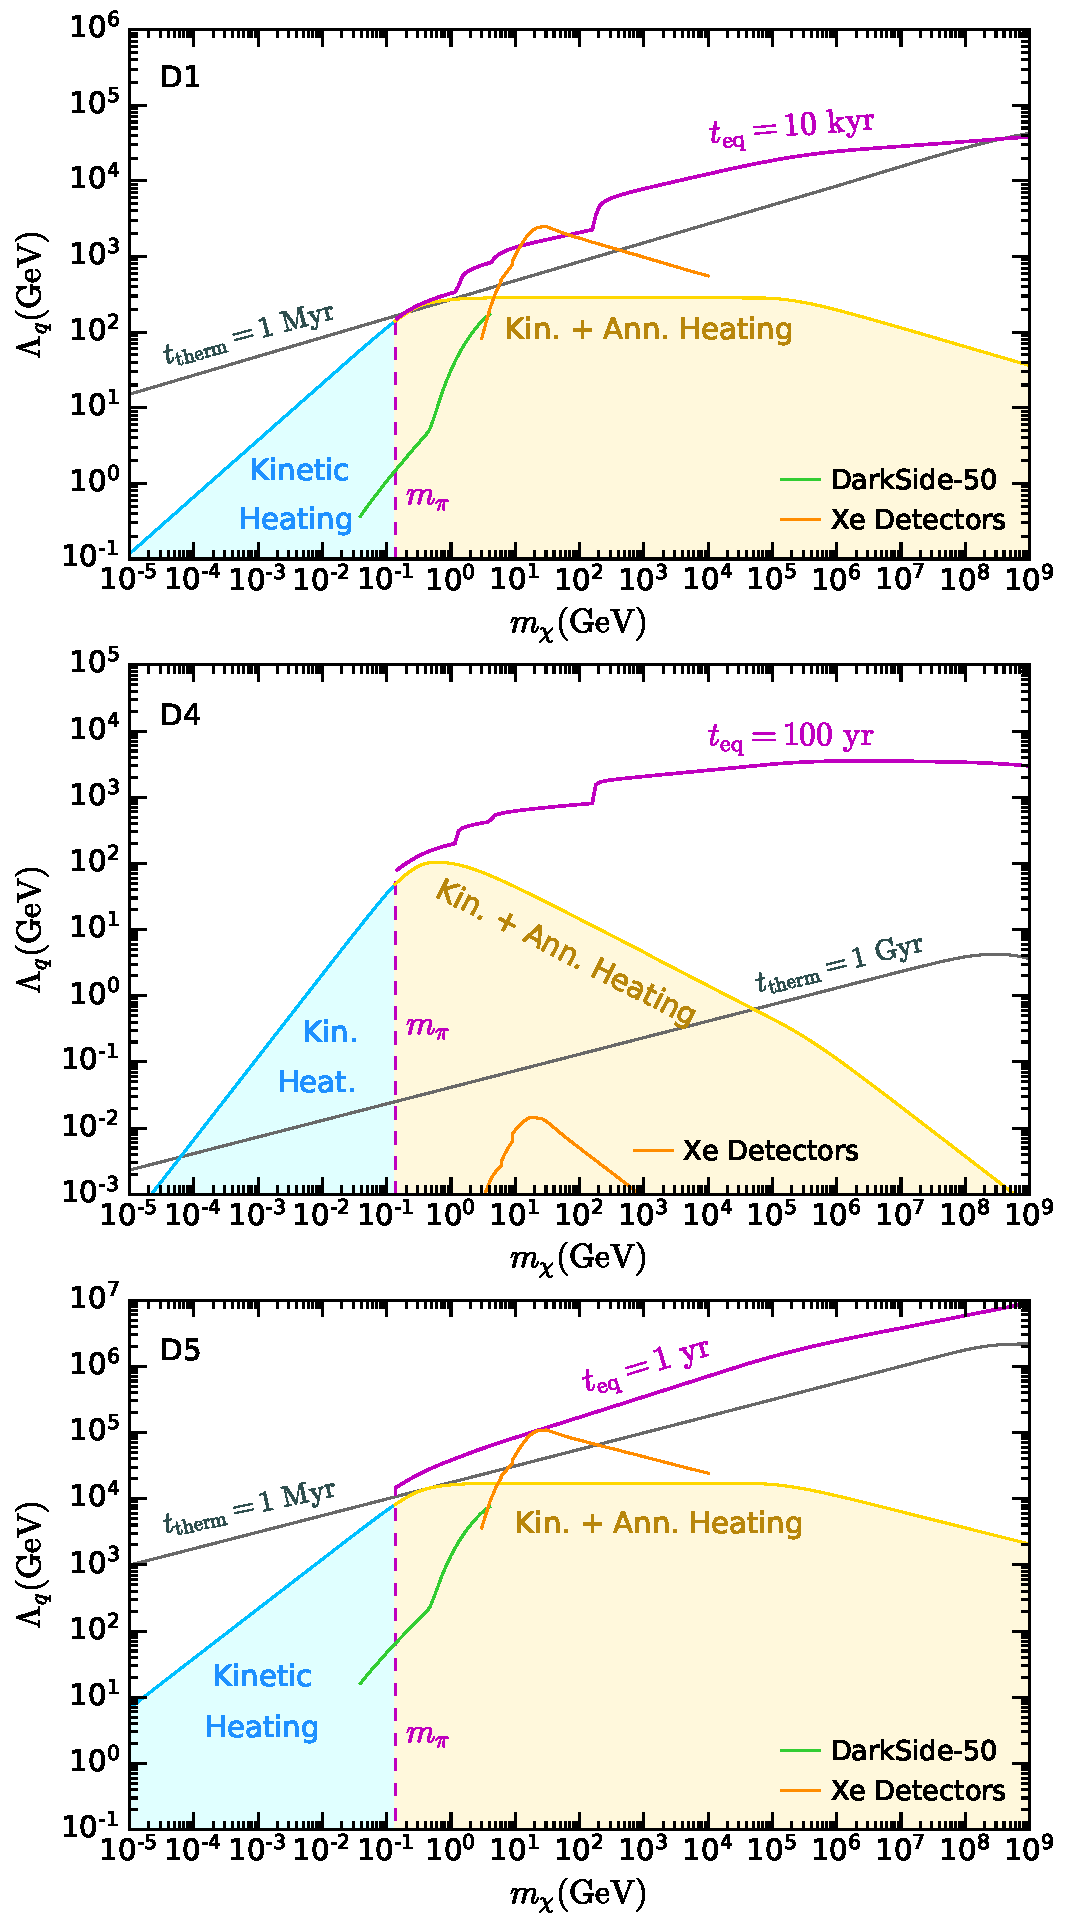
\includegraphics[width=0.6\textwidth]{ann_heat_sensitivity_3ops.pdf}   
    \caption{
    Projected NS heating sensitivity for maximal capture efficiency, for DM-baryon interactions described by operators D1, D4 and D5.  We have used the QMC-2 ($1.5\Msun$) benchmark NS configuration.
    We show the regions where DM kinetic and annihilation heating both contribute to the NS luminosity (yellow) and where kinetic heating alone contributes (light blue).
    Contour lines for capture-annihilation equilibrium (magenta) and thermalisation (grey) are shown for indicative timescales.    
     Lower limits on $\Lambda_q$ from leading  direct detection experiments~\cite{DarkSide:2022dhx_mar_SearchDarkMatterNucleon,XENON:2020gfr_mar_SearchCoherentElastic,PandaX-4T:2021bab_dec_DarkMatterSearch,LZ:2022lsv_jul_FirstDarkMatter} are also shown.  
    }
    \label{ch6:fig:NS_heating}
\end{figure}
%%%%%%%%%%%%%%%%%%%%%%%%%%%%%%%%%%%

We now examine the regions of parameter space where maximal heating can be achieved, for DM-hadron interactions described by the four-fermion operators of Table~\ref{ch6:tab:opers_defn_full}. As the extent of DM-induced heating depends on how efficiently the DM is captured, it is clear that maximal heating corresponds to the case of $f=1$ in Eqs.~\ref{ch6:eq:kinenergy} and~\ref{ch6:eq:massheating}, i.e., when the dark matter scattering cross-section is at or above the geometric limit. 


In Figure~\ref{ch6:fig:NS_heating}, we show the parameters for which the DM deposits its entire kinetic and rest mass energy (yellow region) or only its full kinetic energy (light blue region).  Above these shaded regions, the value of $\Lambda_q$ is too large (and hence the scattering cross-section is too small) for maximal capture.
The overall shape of the shaded regions is dictated by the behaviour of the capture rate. For sub-GeV DM, Pauli blocking suppresses the capture rate, and so smaller $\Lambda_q$ values are required to reach the geometric limit. At large DM mass, $\gtrsim 10^5\GeV$, the capture rate is suppressed because a single collision does not transfer enough energy to result in capture.


We see from the $\teq$ contours (magenta) that capture-annihilation equilibrium, and hence full annihilation heating, is achieved on a timescale much shorter that the NS lifetime, which we take to be $t_\star\sim 1\Gyr$. 
We do not show the contours for the kinetic heating timescale, $t_\mathrm{kin}$, as this is significantly shorter than the age of the star.  Moreover, for masses where DM annihilation to hadrons is possible, $m_\chi>m_\pi$, it is not necessary for kinetic heating to occur before capture-annihilation equilibrium is established, as the total kinetic plus mass energy will be deposited when the DM annihilates. 
For completeness, we include the contours of the thermalisation time (grey). We stress again that the DM does not need to fully thermalise to achieve maximal heating.


To highlight how the sensitivity varies for different interaction types, we show results for operators D1, D4 and D5 in Figure~\ref{ch6:fig:NS_heating}, with the remaining operators presented in Figure~\fixMV{fig:NSheating2}. These operators were chosen because they allow us to compare interactions with and without momentum or velocity-suppressed scattering or annihilation cross-sections. Specifically: 
\begin{itemize}
\item D1 (scalar): unsuppressed scattering cross-section; $p$-wave suppressed annihilation.
\item D4 (pseudoscalar): $q_{\rm tr}^4$ suppressed scattering cross-section; unsuppressed $s$-wave annihilation.
\item D5 (vector): unsuppressed scattering and annihilation cross-sections.
\end{itemize}

Comparing the projected NS heating sensitivity with limits from terrestrial direct detection experiments (shown as green and orange curves in Fig.~\ref{ch6:fig:NS_heating}) we find similar behaviour for D1 and D5. This is expected, as both of these operators give rise to unsuppressed spin-independent DM-nucleon scattering cross-sections. The $p$-wave suppression of the D1 annihilation cross-section increases $\teq$ compared to that for D5; nonetheless, equilibrium is reached relatively quickly compared to $t_\star$.  The D4 (pseudoscalar) interaction has dismal prospects of being observed in direct detection experiments, due to the severe  $q_{\rm tr}^4$ suppression for the scattering of non-relativistic DM. In contrast, NS heating has much greater sensitivity.

Note that the time required for complete thermalisation (grey contours) is much longer for D4 (momentum-suppressed scattering) than for D1 and D5. In fact, for operator D4, full thermalisation is not achieved for most of the interesting parameter space. This illustrates the importance of correctly identifying $\teq$ as the timescale on which full heating is achieved, rather than the much longer $\tth$. 



%%%%%%%%%%%%%%%%%%%%%%%%%%%%%%%%%%%%%%%%%%
\section{Interaction rate in the zero temperature approximation}
\label{ch6:sec:pauliblockingle}
%%%%%%%%%%%%%%%%%%%%%%%%%%%%%%%%%%%%%%%%%%



In this section,  we calculate the interaction rate in the zero temperature approximation for $\Msq = \alpha \, t^n$, where $n=0,1,2$ and $\alpha$ is a constant, in the low energy, Pauli suppressed regime where $K_\chi=E_\chi-m_\chi<\kinFi$. 
We assume the simplest scenario of constant target mass and point-like targets, as justified in Section~\ref{sec:thermstandard}. 

In this approximation, the interaction rate in the energy regime relevant for thermalization is given by~\cite{Bell:2020jou_sep_ImprovedTreatmentDark}
\begin{equation}
\Gamma^{-}(K_\chi,\Tstar=0) \propto \, \frac{1}{2^7\pi^3 K_\chi k }  \int_0^{K_\chi} q_0 dq_0 \,\, \int \frac{t_E^n dt_E }{\sqrt{q_0^2+t_E}}\Theta(\kinFi-q_0),
\label{ch6:eq:gammafinal}
\end{equation}
where $t_E=-t$,   and 
\begin{equation}
\int \frac{t_E^n dt_E }{\sqrt{q_0^2+t_E}} = 2D_n(q_0^2,t_E)\sqrt{q_0^2+t_E}.
\end{equation}
The $D_n$  functions can be found in Appendix B of  Ref.~\cite{Bell:2020jou_sep_ImprovedTreatmentDark}. 
As we shall see, the integration intervals in Eq.~\ref{ch6:eq:gammafinal} depend on whether or not Pauli blocking suppresses any part of the thermalization process.
In both cases, we can find simple analytic approximations to these integrals. 
The minimal DM mass for which Pauli blocking is never in effect is denoted by $\mcrit$. 
  
We first consider the case where $m_\chi \lesssim \mcrit$. 
For the cases of $\mu \ll \kinFi/K_\chi$ or $\mu \gg K_\chi/\kinFi$, 
$\Gamma^{-}$ at first order in $K_\chi$ is given by
% 
\begin{align}
\Gamma^{-}(K_\chi) &\sim \frac{\alpha}{2^7\sqrt{2}\pi^3m_\chi^{3/2}K_\chi^{1/2}}\int_0^{K_\chi}q_0 dq_0 \left(\int_{t_{E}^{-}}^{t_{E}^{+}} \frac{t_E^n dt_E }{\sqrt{q_0^2+t_E}} \right)\\
&= \frac{\alpha}{2^6\sqrt{2}\pi^3m_\chi^{3/2}K_\chi^{1/2}}\int_0^{K_\chi}q_0 dq_0 \left(\sqrt{q_0^2+t_E^{+}}D_n(q_0^2,t_E^{+})-\sqrt{q_0^2+t_E^{-}}D_n(q_0^2,t_E^{-})\right), \label{ch6:eq:intratelowe}
\end{align}
% 
where $t_E^\pm$ are defined in Ref.~\cite{Bell:2020jou_sep_ImprovedTreatmentDark}. 
For matrix elements independent of $t$ ($n=0$), we have $D_0(q_0^2,t_E^{\pm})=1$  and this result simplifies to
% 
\begin{align}
\Gamma_{n=0}^{-}(K_\chi) 
&\sim  \frac{|\overline{\mathcal{M}}|^2}{2^6\pi^3m_\chi}\int_{0}^{K_\chi} dq_0 q_0 \left[\sqrt{2\left(1+\sqrt{1-\frac{q_0}{K_\chi}}\right)-\frac{q_0}{K_\chi}}-\sqrt{2\left(1-\sqrt{1-\frac{q_0}{K_\chi}}\right)-\frac{q_0}{K_\chi}}\right] \nonumber \\
&= \frac{|\overline{\mathcal{M}}|^2}{120\pi^3m_\chi}K_\chi^2.
\end{align}
% 
We can rewrite the previous expression in terms of the DM-baryon scattering cross-section using the following expression
\begin{equation}
\sigma_{i\chi}^{n=0} = \frac{\Msq}{16\pi m_i^2 (1+\mu)^2}, 
\label{ch6:eq:intraten0}
\end{equation}
giving the interaction rate at first order in $K_\chi$
\begin{equation}
\Gamma_{n=0}^{-}(K_\chi)  \sim \frac{2 m_i}{15}\frac{(1+\mu)^2}{\mu}K_\chi^2 \sigma_{i\chi}^{n=0}.
\end{equation}
This result has the same $K_\chi$ and $\mu$ scaling as that of Ref.~\cite{Bertoni:2013bsa_dec_DarkMatterThermalization}.



Performing a similar analysis for $\Msq=\alpha (-t)^n$, $n=1,2$, 
we find 
\begin{equation}
\Gamma_{n=1}^{-}(K_\chi) 
\sim \frac{2\alpha }{105\pi^3}K_\chi^3,\qquad 
\Gamma_{n=2}^{-}(K_\chi) 
\sim \frac{4\alpha }{63\pi^3}m_\chi K_\chi^4. 
\end{equation}
The expressions for the cross-sections for $n=1,2$ are 
\begin{equation}
\sigma^{n=1}_{i\chi} = \frac{\alpha}{16\pi m_i^2(1+\mu)^2}t_{max},\qquad
\sigma^{n=2}_{i\chi} = \frac{4}{3}\frac{\alpha}{16\pi m_i^2(1+\mu)^2}t_{max}^2.   
\end{equation}
These cross-sections must be normalized to sensible momentum transfer. We take this reference point to be the surface of the star, such that 
\begin{equation}
      t_{max} \sim \frac{4m_\chi^2}{1+\mu^2}\frac{1-B(\Rstar)}{B(\Rstar)}.   
\end{equation}
The interaction rates for $n=1,2$ can then be written as
\begin{eqnarray}
    \Gamma_{n=1}^{-}(K_\chi) &\sim& \frac{8}{105 \pi^2} \frac{(1+\mu)^2(1+\mu^2)}{\mu^2} \sigma_{\rm surf} \, K_\chi^3 \frac{B(\Rstar)}{1-B(\Rstar)}, \label{ch6:eq:intraten1}\\
\Gamma_{n=2}^{-}(K_\chi) &\sim& \frac{1}{21 \pi^2} \frac{(1+\mu)^2(1+\mu^2)^2}{\mu^3} \frac{\sigma_{\rm surf}}{m_i} \, K_\chi^4\left[\frac{B(\Rstar)}{1-B(\Rstar)}\right]^2.
\label{ch6:eq:intraten2}
\end{eqnarray}


We now look at the interaction rate in the super-heavy DM mass regime, $m_\chi \gtrsim \mcrit$.
The exact value of $\mcrit$ will depend on the NS configuration. However, we can take some typical values relevant to thermalization to give an estimate of its value. Taking $K_\chi=10^3\K$, $\kinFi=200\MeV$, we see that
\begin{equation}
    m_\chi \ge \frac{2\kinFi(2m_i+\kinFi)}{ K_\chi} \sim \frac{4\kinFi m_i}{K_\chi} = m_\chi^{\rm crit}\sim 9.65\times10^9\GeV. 
\end{equation}
The maximum energy transfer in this regime will always be $\qomax<K_\chi$, with
\begin{equation}
    \qomax\sim K_\chi\left[2\sqrt{\frac{m_\chi^{\rm crit}}{m_\chi }} - \frac{m_\chi^{\rm crit}}{m_\chi } +\mathcal{O}\left(\left(\frac{m_\chi^{\rm crit}}{m_\chi}\right)^{\frac{3}{2}}\right)\right].
 \end{equation}
Performing a similar analysis as the $m_\chi \lesssim \mcrit$ regime leads to the following expression for $\Gamma^-$,
\begin{equation}
\Gamma^{-}(K_\chi) \sim \frac{|\overline{\mathcal{M}}|^2}{2^7\sqrt{2}\pi^3m_\chi^{3/2}K_\chi^{1/2}}\int_0^{	\qomax}q_0 dq_0 \left(\int_{t_{E}^{-}}^{t_{\mu^-}^{+}} \frac{t_E^n dt_E }{\sqrt{q_0^2+t_E}} \right),  
\end{equation} 
where $t_{\mu^-}^+$ is defined in Ref.~\cite{Bell:2020jou_sep_ImprovedTreatmentDark}. 
For the simplest case of constant $|\overline{\mathcal{M}}|^2$ this results in 
\begin{align}
\Gamma^{-}_{n=0}(K_\chi) & \sim  
\frac{K_\chi \kinFi |\overline{\mathcal{M}}|^2}{24\pi^3\mu^2m_i}\left[\sqrt{\frac{m_\chi^{\rm crit}}{m_\chi}}+\mathcal{O}\left(\frac{m_\chi^{\rm crit}}{m_\chi}\right)\right] \nonumber\\
& = \frac{|\overline{\mathcal{M}}|^2(m_i\kinFi)^{3/2}}{12 \pi^3m_\chi^{5/2}}K_\chi^{1/2}.\label{ch6:eq:intraten0largem}
\end{align}



%%%%%%%%%%%%%%%%%%%%%%%%%%%%%%%%%%%%%%%%%%%%%%%%%%%%%%%%%%%%%%%%%%%%%%%%%%%%%%%%%%%%
%%%%%%%%%%%%%%%%%%%%%%%%%%%%%%%%%%%%%%%%%%%%%%%%%%%%%%%%%%%%%%%%%%%%%%%%%%%%%%%%%%%%
\section{Thermalization of super-heavy DM}
\label{ch6:sec:thermsuperheavy}
%%%%%%%%%%%%%%%%%%%%%%%%%%%%%%%%%%%%%%%%%%%%%%%%%%%%%%%%%%%%%%%%%%%%%%%%%%%%%%%%%%%%
%%%%%%%%%%%%%%%%%%%%%%%%%%%%%%%%%%%%%%%%%%%%%%%%%%%%%%%%%%%%%%%%%%%%%%%%%%%%%%%%%%%%



For DM that is heavier than the critical mass  $m_\chi\gtrsim m_\chi^{\rm crit}$,
the energy lost in each scatter is a tiny fraction of the total DM kinetic energy. Moreover, the average time between collisions is typically on the order of fractions of a second. This warrants the use of a continuous approximation in this regime rather than performing the discrete summation. The thermalization time is then found by integrating the rate at which the DM kinetic energy changes, 
\begin{equation}
    \frac{dK_\chi}{dt} = -\Gamma^{-}(K_\chi) \langle\Delta K_\chi\rangle,  
    \label{ch6:eq:contttherm}
\end{equation}
from the initial kinetic energy, $K_\chi=m_\chi\left(\frac{1}{\sqrt{B(r)}}-1\right)$, to the final value $T_{\rm eq}\ll m_\chi$. For a constant cross-section ($n=0$), we substitute  Eqs.~\ref{ch6:eq:intraten0largem} and \ref{ch6:eq:aveElossn0largem} into the expression above leading to
\begin{equation}
    \tthn{0} \sim \frac{9 \pi^2 m_\chi}{8 (\mbeff)^2 \kinFi^2 \sigma_{i\chi}^{n=0}}\log\left[\frac{m_\chi}{T_{\rm eq}}\left(\frac{1}{\sqrt{B(\Rstar)}}-1\right)\right].
    \label{ch6:eq:tthemheavy0}
\end{equation}
Taking the final temperature to be $T_{\rm eq}=10^3\K$ and $B(\Rstar)=0.5$, this yields 
\begin{equation}
    \tthn{0} \sim 1.7  \yrs \left(\frac{m_\chi }{10^{10}\GeV}\right)\left(\frac{0.5\;m_n}{\mbeff(0)}\right)^{2}\left(\frac{0.2\GeV}{\kinFi(0)}\right)^{2}\left(\frac{10^{-45}\cm^2}{\sigma_{i\chi}^{n=0}}\right).    
\end{equation}
%
Repeating for $d\sigma\propto t^n$ ($n=1,2$), we calculate the thermalization time for $n=1$ to be
\begin{eqnarray}
    \tthn{1} &\sim& \frac{9\pi^2 m_\chi}{ 64 \mbeff \kinFi^3 \sigma_{i\chi}^{n=1}}\left[\frac{1-B(\Rstar)}{B(\Rstar)}\right] \log\left[\frac{m_\chi}{T_{\rm eq}} \left(\frac{1}{\sqrt{B(\Rstar)}}-1\right)\right],\\
    &\sim& 3.5 \yrs\; \left(\frac{m_\chi}{10^{10} \GeV}\right)\left(\frac{0.5\;m_n}{\mbeff(0)}\right) \left(\frac{0.2\GeV}{\kinFi(0)}\right)^{3}\left(\frac{10^{-45}\cm^2}{\sigma_{i\chi}^{n=1}}\right),
\end{eqnarray}
and that for $n=2$ to be
\begin{eqnarray}
    \tthn{2} &\sim& \frac{5 \pi^2 m_\chi}{ 32 \kinFi^4\sigma_{i\chi}^{n=2}} \left[\frac{1-B(\Rstar)}{B(\Rstar)}\right]^2 \log\left[\frac{m_\chi}{T_{\rm eq}}\left(\frac{1}{\sqrt{B(\Rstar)}}-1\right)\right],\\
    &\sim& 3.5 \yrs \left( \frac{m_\chi}{10^{10} \GeV}\right) \left(\frac{0.2\GeV}{\kinFi(0)}\right)^{4}\left(\frac{10^{-45}\cm^2}{\sigma_{i\chi}^{n=2}}\right). 
\end{eqnarray}







%%%%%%%%%%%%%%%%%%%%%%%%%%%%%%%%%%%%
\section{Thermalization time for $s$- and $t$-dependent interactions}
\label{ch6:sec:sdeptherm}
%%%%%%%%%%%%%%%%%%%%%%%%%%%%%%%%%%%%


In Section~\ref{sec:thermstandard}, we assumed $\Msq\propto t^n$ when deriving analytical approximations for the thermalization timescale. To understand the behavior of the thermalization time for the operators in Table.~\ref{ch6:tab:opers_defn_full}, we can make use of the results for $t^n$ dependent interactions. For cross-sections that are linear combinations of different powers of $t$, we can approximate the thermalization time using the previous results in the following way
\begin{align}
\Msq &= a_0 + a_1 t + a_2 t^2,\\
\sigma &= a_0\sigma_0 + a_1 \sigma_1 + a_2 \sigma_2,\\
\frac{1}{\tth} &\sim \frac{a_0}{ \tthn{0}(\sigma_{i\chi}=\sigma_0)} + \frac{a_1} {\tthn{1}(\sigma_{i\chi}=\sigma_1)} 
 + \frac{a_2}{  \tthn{2}(\sigma_{i\chi}=\sigma_2)}. 
\label{ch6:eq:ttherm_weighted}
\end{align}
Hence, the inverse of the thermalization time will be given by a weighted linear combination of the inverse times for each contribution. As higher powers of $t$ require significantly longer thermalization times, for coefficients of similar size, the resulting sum will be dominated by the lowest power of $t$ appearing in  $\Msq$.  We can thus identify the dominant terms for operators D1-D4  based on power counting, which we have listed in Table~\ref{ch6:tab:opers_defn_full}.

 For $s$-dependent amplitudes, we can in principle use the interaction rates calculated  in Appendix A of Ref.~\cite{Bell:2020lmm_mar_ImprovedTreatmentDark}, perform a series expansion in $K_\chi$  and repeat the same procedure outlined in Section~\ref{sec:thermstandard} for $s$-independent matrix elements. Interestingly, we find that for the purpose of calculating the thermalization time, there is an easier way to obtain the correct result. One can indeed check that, at zero order in $\kinFi/\mbeff$, the resulting time for $s^1, s^2$ is equivalent to the constant case, with the matrix element calculated by setting 
\begin{equation}
    s\rightarrow (m_\chi+\mbeff)^2,
    \label{ch6:eq:ssubst}
\end{equation}
while the $s t $ case has a result equivalent to the $t$ case, with the matrix element calculated using the same substitution. This is, in practice, equivalent to setting both the DM and neutron targets at rest. There is, however, an important exception, when it comes to calculating the thermalization time of a linear combination of these terms. In particular, when the amplitudes at order $\mathcal{O}(t^0)$, are proportional to combinations of $1,s,s^2$ such as
\begin{gather}
s-(m_\chi+\mbeff)^2,\nonumber\\
\left[s-(m_\chi+\mbeff)^2\right]^2,\nonumber\\
\left[s-(\mbeff)^2-m_\chi^2\right]^2-4(\mbeff)^2 m_\chi^2.\label{ch6:eq:m2veldep}
\end{gather}
All these combinations give a null result after applying substitution \ref{ch6:eq:ssubst}. In such a case, one may think that the dominant term is given by some remaining $t^n$ term. It is worth noting that the expressions in  Eq.~\ref{ch6:eq:m2veldep}  appear in operators that, at low energy, are known as  velocity-dependent, because their matrix elements are proportional to positive even powers of the DM-target relative speed. Consequently, it is important not to neglect the motion of the targets in the neutron star, moving at relativistic speeds that are of the order of the Fermi velocity $v_F^2=2\kinFi/\mbeff$. In those cases, one should instead set $s$ to\footnote{We assume that $\mu\gg \mbeff/m_\chi^{\rm crit}$ when making this substitution.}
\begin{equation}
    s\rightarrow (m_\chi+\mbeff)^2+2m_\chi\kinFi.
    \label{ch6:eq:ssubstmu}
\end{equation}



In summary, operators D5, D8 and D9 can be safely expanded using \ref{ch6:eq:ssubst}, while operators D6, D7 and D10 have velocity-dependent amplitudes and require Eq.~\ref{ch6:eq:ssubstmu}. 
The dominant terms for each operator can be found in Table~\fixMV{Add the dominant terms in a new table}. 
For equal values of the leading term in $\Msq$, the thermalization time for each operator will be the same as the relevant $t^n$ power law. 


%%%%%%%%%%%%%%%%%%%%%%%%%%%%%%%%%%%%%%%%%%%%%%%%%%%%%%%%%%%%%%%
\section{Temperature distribution of captured dark matter}
\label{ch6:sec:minTempDerivation}
%%%%%%%%%%%%%%%%%%%%%%%%%%%%%%%%%%%%%%%%%%%%%%%%%%%%%%%%%%%%%%



As seen in Fig.~\ref{ch6:fig:thermtime}, interactions that depend on the momentum transfer, namely $d\sigma \propto t^n$ with $n = 1,2$, there are regions of the DM mass parameter space where thermalization does not occur within the age of the star. For the DM masses and NS temperatures of interest, this region of non-thermalization always occurs in the $m_\chi\ll \mcrit$ regime.
From Eqs.~\ref{ch6:eq:thermtimen0}, \ref{ch6:eq:thermtimen1} and \ref{ch6:eq:thermtimen2},  we can estimate the time required for the DM to reach a kinetic energy $K_\chi$ 
\begin{equation}
    t_{K_\chi} \propto \frac{1}{K_\chi^{n+2}}.
\end{equation}
% 
If the DM does not thermalize within the age of the star, it will instead reach a minimum temperature, $K_\chi^{\mathrm{min}}$.  Comparing the time required to achieve this temperature to the thermalization time, $\tth$ i.e. to have reached the equilibrium temperature $\Teq$, we find 
\begin{equation}
    \frac{t_{K_\chi^\mathrm{min}}}{\tth}  \sim \left( \frac{\Teq}{K^{\rm min}_\chi} \right)^{n+2}. 
\end{equation}
Accounting for the case where the DM reaches thermalization, we can write $K_\chi^\mathrm{min}$
\begin{align}
    K^{\rm min}_\chi & \sim \Teq \left(\max\left[ 1,\frac{\tth}{t_{K_\chi^\mathrm{min}}}\right ]\right)^{\frac{1}{n + 2}}\\
           & \approx \Teq \left( 1 + \frac{\tth}{t_{K_\chi^\mathrm{min}}}\right )^{\frac{1}{n + 2}}. 
\end{align}
The population of captured DM will have a distribution of energies at any given time, with this distribution being peaked at this minimum energy.
As the orbital periods of the DM will be much shorter than the average time between interactions, the DM will be able to virialize between each interaction. Therefore, we can treat the DM as being contained within an isothermal sphere with temperature $K^{\rm min}_\chi > \Teq$. 

Finally, it is worth noting that at times  $t>\tth$, even though the thermalization condition has been reached, the captured DM would consist of two components: a fraction of it (whose amount depends on time) would be in thermal equilibrium with the NS at temperature $T_{\rm eq}$; and another component still in the cooling down process. Assuming a  capture rate constant over time, the fraction of thermalized DM is 
\begin{equation}
    f_{\rm therm}(t) = \frac{t-t_{\rm therm}}{t}.
\end{equation}



%%%%%%%%%%%%%%%%%%%%%%%%%%%%%%%%%%%%%%%%%%%%%%%%%%%%%%%%%%%%%%%
\section{Quark-level vs hadron-level annihilation cross-sections}
\label{ch6:sec:quarkhadron}
%%%%%%%%%%%%%%%%%%%%%%%%%%%%%%%%%%%%%%%%%%%%%%%%%%%%%%%%%%%%%%%

The annihilation cross-sections shown in Table~\ref{ch6:tab:annCS} are for DM annihilation to quark final states.  More properly, we should consider the hadron-level annihilation cross-section.
However, we are primarily concerned with the capture-annihilation equilibrium timescale, and not the details of the annihilation process. Therefore, if the annihilation rate to hadrons is not significantly different from the quark level result, this subtlety can be avoided. 

To check the validity of the quark-level approximation, we estimate the annihilation rate to hadrons, working at lowest order in Chiral Perturbation Theory. We use couplings to the meson octet obtained from  Ref.~\cite{Kumar:2018heq_dec_IndirectDetectionSubGeV}; for annihilation to baryons, the operators listed in Table~\ref{ch6:tab:opers_defn_full} are used. 
For DM masses in the range $m_\pi < m_\chi \lesssim m_{\rm charm} = 1.27\GeV$, we find that the cross-section for annihilation to hadrons differs by less than an order of magnitude than that for annihilation to quarks. For larger DM mass, the difference is negligible. Therefore, to simplify the discussion, we consider DM annihilation to quark final states for DM masses above the pion mass.


Below the pion mass, the only kinematically allowed DM annihilation channels would be to leptons or photons. The size of the DM couplings to these states would, in general, be unrelated to the DM-quark couplings we have assumed. (They are expected to be non-zero, because they would be induced at loop level~\cite{Bell:2019pyc_jun_CaptureLeptophilicDark}, even if absent at tree level.)
However, due to the considerable Fermi energies of the electrons and muons near the centre of the NS, these channels will be Pauli blocked for the whole DM mass range below $m_\pi$, forbidding these annihilations from occurring. To remain as model-independent as possible, we will not consider lepton and photon annihilation channels.

Figure~\ref{ch6:fig:ann_xs_plots} shows $t_{\rm eq}$ contour lines in the $\Lambda_q-m_\chi$ plane for the NS benchmark model QMC-2, $\Tstareq=1000\K$ and two representative operators D7 (left) and D8 (right). 
Operators whose thermally averaged annihilation cross-section $\sigmav$ has a  $m_f/m_\chi$ leading order term, namely D1-D4 and D8 (see Table~\ref{ch6:tab:annCS}), exhibit a sudden change in the slope wherever a new annihilation channel opens (see dotted lines on the right panel of Fig.~\ref{ch6:fig:ann_xs_plots}). Note that the higher the cutoff scale $\Lambda_q$, the lower the scattering and annihilation cross-sections, resulting in a larger $t_{\rm eq}$ timescale. For lower $\Teq$ temperatures, DM requires more time to reach both equilibrium conditions, thermalization and capture-annihilation. The variation of these results with respect to the NS configuration amounts at most to a factor of $\sim2$ in the $t_{\rm eq}$ contours (see shaded regions in the left panels) from the lightest configuration (QMC-1, $1\Msun$) to the heaviest (QMC-3, $1.9\Msun$) for most operators, with the sole exception of D4 for which this factor rises up to $\sim 2.4$. 

%%%%%%%%%%%%%%%%%%%%%%%%%%%%%%
\begin{figure}[t!bp]
    \centering
    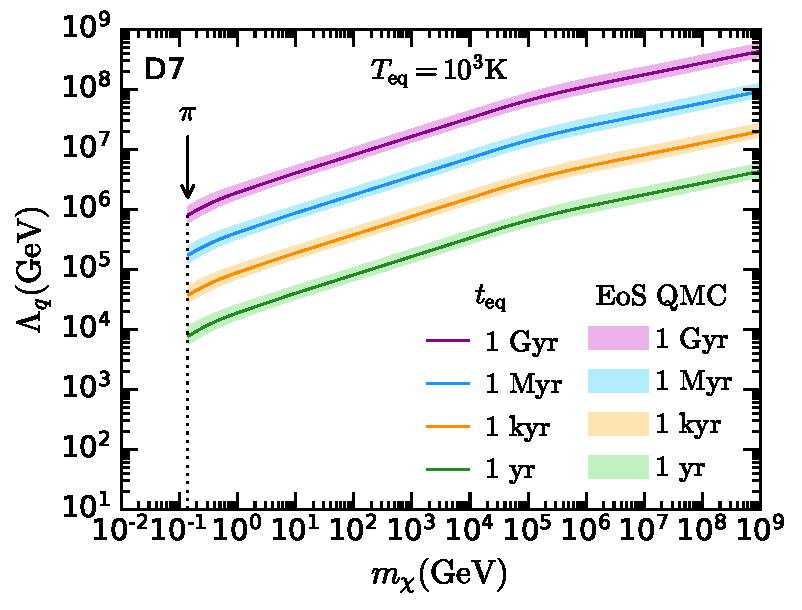
\includegraphics[width = 0.496\textwidth]{D7_Lambda_mdm_teq.pdf}
    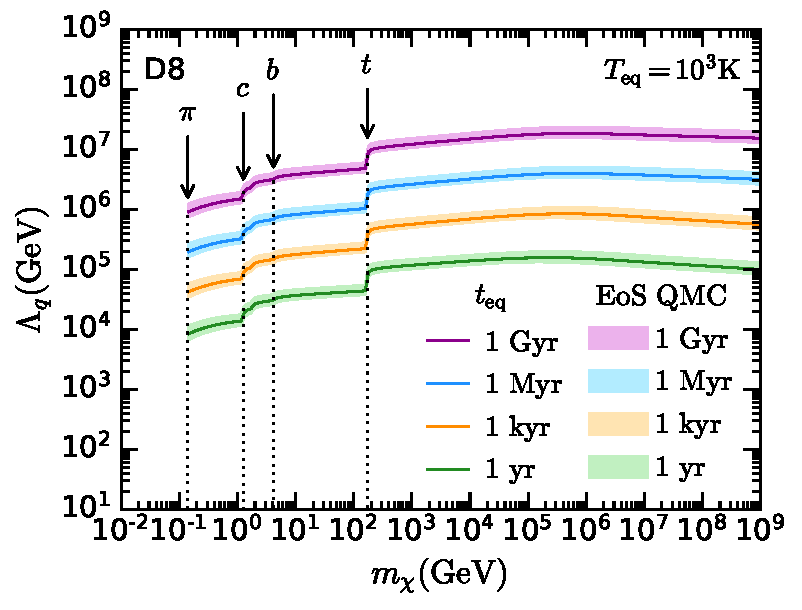
\includegraphics[width = 0.496\textwidth]{D8_Lambda_mdm_teq.pdf}    
    \caption{
    Contours of the capture annihilation timescale, $t_{\rm eq}$,  in the $\Lambda_q-m_\chi$ plane for operators D7 (left) and D8 (right) and $\Tstareq=1000\K$. 
    Solid lines represent the calculation for the NS benchmark model QMC-2, and shaded regions denote the variation with the NS choice for the QMC EoS family. 
    Dotted lines in the right panel indicate the mass thresholds for various annihilation channels.  
    }
    \label{ch6:fig:ann_xs_plots}
\end{figure}
%%%%%%%%%%%%%%%%%%%%%%%%%%%%%%%%%%%%%%


%%%%%%%%%%%%%%%%%%%%%%%%%%%%%%%%%%%%%%%%%%%%%%%%%%%%%%%%%%%%%%%
\section{Capture-annihilation equilibrium for EFT operators}
\label{ch6:sec:resultsEFTop}
%%%%%%%%%%%%%%%%%%%%%%%%%%%%%%%%%%%%%%%%%%%%%%%%%%%%%%%%%%%%%%%

\begin{figure*}
    \centering
    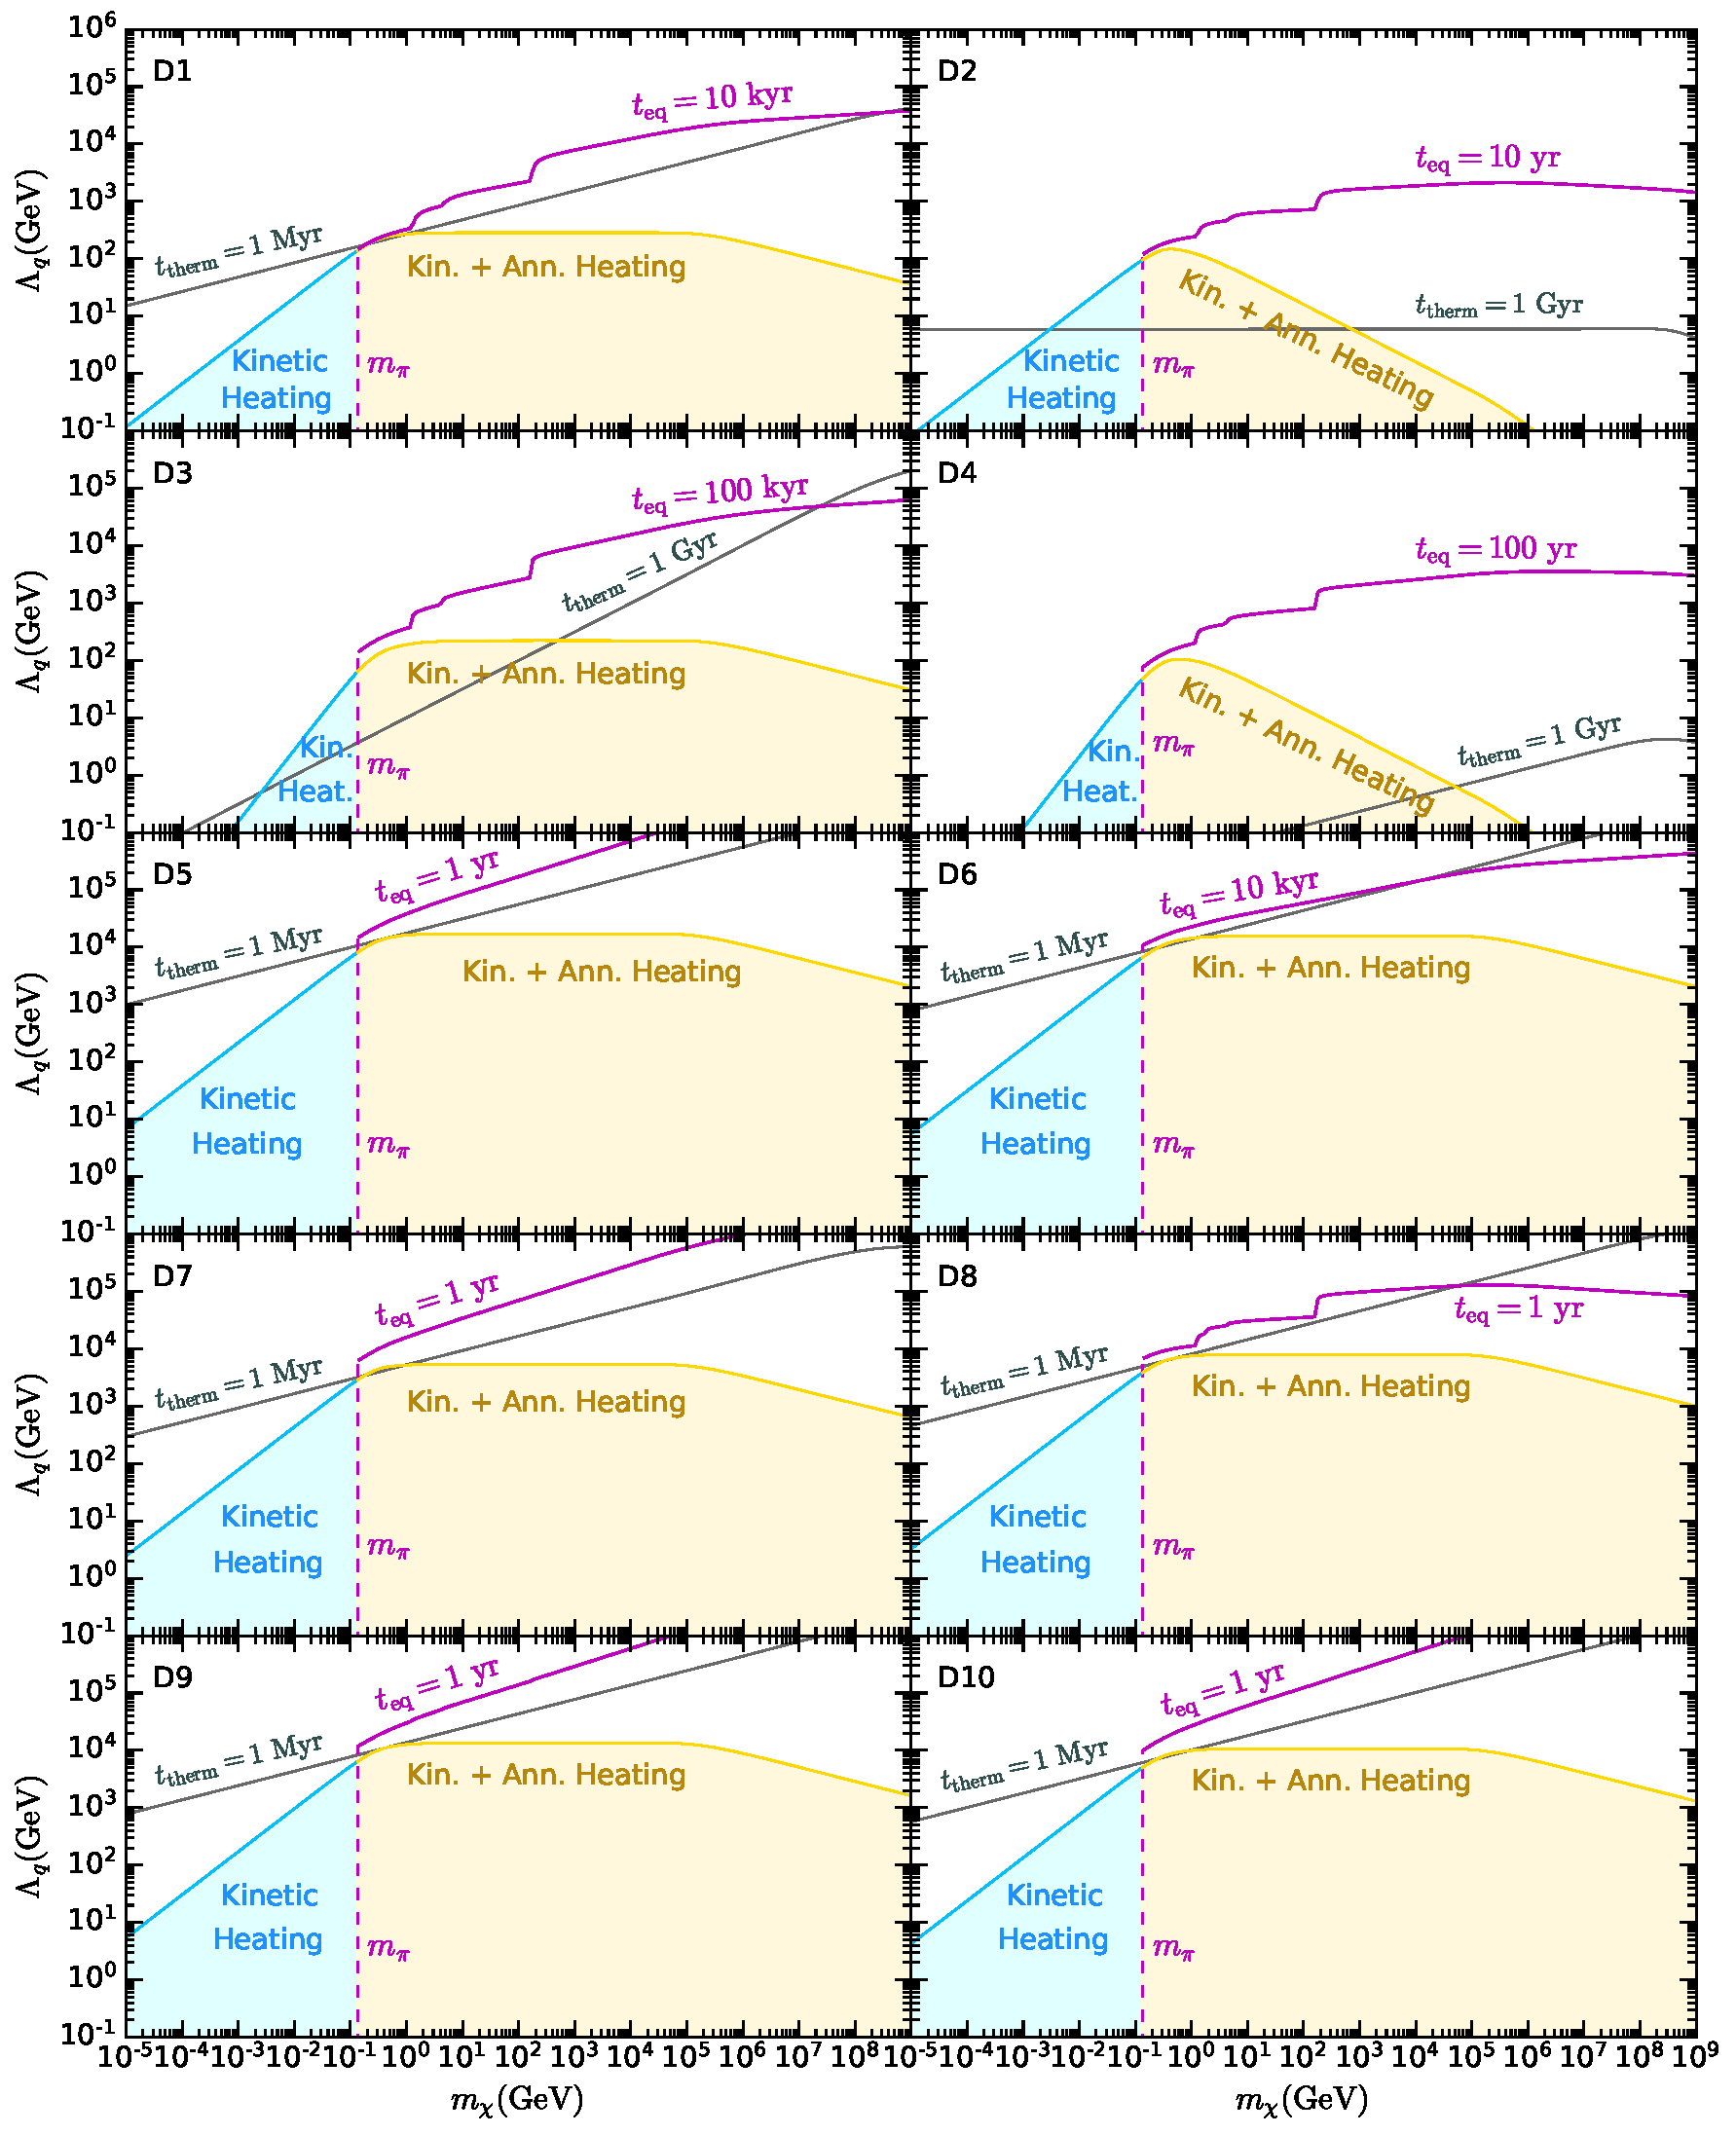
\includegraphics[width=\textwidth]{ann_heat_sensitivity.pdf}    
    \caption{Projected NS heating sensitivity for maximal capture efficiency, for the full set of DM-baryon interactions described by the EFT operators of Table~\ref{ch1:tab:opers_defn_full}. We have used the QMC-2 ($1.5\Msun$) benchmark NS configuration.  
    Color coding as in Fig.~\ref{ch6:fig:NS_heating}. 
    }
    \label{ch6:fig:NS_heating2}
\end{figure*}



In Fig.~\ref{ch6:fig:NS_heating2}, we show isocontours of maximal capture (yellow and light blue lines) and capture-annihilation equilibrium (magenta lines) timescale in the $\Lambda_q-m_\chi$ plane for all  EFT operators.  
Values of $\Lambda_q$ below the $t_{\rm eq}$ lines result in smaller capture-annihilation equilibrium timescales. 
We can see in Fig.~\ref{ch6:fig:NS_heating} that for all operators the $t_{\rm eq}$ timescale is always smaller than the time required for captured DM to thermalize. Captured DM achieves the steady state condition in a timescale as short as $\sim1\yr$ (D1, D6-D10) or as long as $10^5\yr$ (D3). 
Note that the displayed lines for the $t_{\rm eq}$ are the values for which the entire parameter space relevant for capture reaches equilibrium with annihilation. 

For D1 and D6-D10, we observe that captured DM achieves thermal equilibrium in less than $\sim 1\Myr$ (grey lines). 
On the other hand, as expected from Fig.~\ref{ch6:fig:thermtime} captured DM whose interactions are momentum suppressed, namely operators D2-D4, would never thermalize to the temperature expected from DM-induced heating in $1\Gyr$, or even in less than the age of the 
Universe,
with the sole exception of the corner region of very light DM $m_\chi\lesssim 2\MeV$ and an even narrower corner of the parameter space for D4. 

Therefore, for all EFT operators,  the energy released in the annihilation process adds up to the energy deposited via capture increasing the DM-induced heating  
for $m_\chi\gtrsim m_\pi$ (yellow shaded area). 
Recall that we have made no assumptions about the energy scale that controls DM interactions with leptons. 
For DM of mass below $m_\pi$ (light blue lines), at least kinetic heating is expected to contribute to the star luminosity.  

  